\documentclass[a4paper,11pt]{report}

% Diese Datei ist fast vollständig von der Maturaarbeit
%
% Programmierung eines Generators für Trennlinien
% bzw. Schnittkurven von Puzzleteilen
%
% vorgelegt von Luca Bosin im Januar 2019, übernommen.
%
% Ihm sei herzlich gedankt.


% ======== START VON PAKETE LADEN =========
\usepackage[utf8]{inputenc}       % Utf8 Zeichensatz
\usepackage[T1]{fontenc}          % Schriftenkodierung
\usepackage[lighttt]{lmodern}     % Schriftart
\usepackage{amsmath}              % Mathematische Formeln
\usepackage[normalem]{ulem}       % Durchgestrichener Text
\usepackage{xcolor}               % Farbiger Text
\usepackage{verbatim}             % Text ohne Formatierung
\usepackage{listings}             % Code mit Formatierung
\usepackage{csquotes}             % Kontextsensitive Zitatanlage
\usepackage{caption}              % Erweiterte Beschriftungen
\usepackage{subcaption}           % Unterbeschriftungen
\usepackage{geometry}             % Seitenränder
\usepackage{setspace}             % Zeilenabstand
\usepackage{fancyhdr}             % Header und Footer
\usepackage{graphicx}             % Grafiken
\usepackage{svg}                  % SVG Grafiken
\usepackage{booktabs}             % Tabellen
\usepackage{tabularx}             % Breite von Boxen
\usepackage[style=ieee]{biblatex} % Referenzen
\usepackage{hyperref}             % Hyperlinks im PDF-Dokument
\usepackage{hyperxmp}             % Metadaten im PDF-Dokument
\usepackage{makeidx}
\usepackage{wrapfig}
\makeindex
% ========= ENDE VON PAKETE LADEN =========


% ==== START VON DOKUMENTEIGENSCHAFTEN ==== (Dokument)
\title                   % Titel festlegen
{A Research on Piezoelectric Elements as a new sustainable energy resource with the emphasis on Roads, Railways and Pathways}
\makeatletter            % Erlaubt das Auslesen der obigen Eigenschaften
\let\papertitle\@title   % Titel in \papertitle speichern
\makeatother
\def\papertype           % Art dieser Arbeit in \papertype speichern
{Extended Essay}
\def\paperquestion
{Are piezoelectric elements a new renewable energy resource applicable in roads, railways, and pathways?}
\def\papersubject
{Physics}
% Achtung: Schlüsselwörter sind weiter unten definiert!
% ==== ENDE VON DOKUMENTEIGENSCHAFTEN =====



% =========================================



% ======= START VON TITEL ANPASSEN ======== (Beschriftungen)
% ======== ENDE VON TITEL ANPASSEN ========



% === START VON SCHRIFTPROBLEME BEHEBEN === (Schriftart)
% Die Schreibmaschinen-Schrift lädt nur den normalen Stil, nicht den fetten oder den kursiven
\ttfamily
\DeclareFontShape{T1}{lmtt}{m}{it}{<->sub*lmtt/m/sl}{}
% === ENDE VON SCHRIFTPROBLEME BEHEBEN ====



% ========= START VON CODEBLÖCKE ========== (Codeblöcke)
\lstset{
  frame=tb,                         % Rahmenlinien (tb = top,bottom)
  language=Java,                    % Programmiersprache (für Syntax-Hervorhebung)
  showstringspaces=false,           % Leerzeichen in Strings ausblenden
  basicstyle=\small\ttfamily,       % Style des Codes
  numbers=left,                     % Position der Zeilennummern
  numberstyle=\tiny\textbf,         % Style der Zeilennummern
  keywordstyle=\textbf,             % Style der Schlüsselwörter
  commentstyle=\color{gray}\textit, % Style der Kommentare
  columns=fullflexible,             % Zeilenumbrüche: Bis an Seitenrand
  breaklines=true,                  % Zeilenumbrüche: Erlauben von Zeilenumbrüchen
  breakatwhitespace=true,           % Zeilenumbrüche: Erlauben von Zeilenumbrüchen bei Leerzeichen
  tabsize=4,                        % Grösse der Tabulatoren (Hard-Tab)
}
% Unterstützung von Sonderzeichen
\lstset{literate=
  {á}{{\'a}}1 {é}{{\'e}}1 {í}{{\'i}}1 {ó}{{\'o}}1 {ú}{{\'u}}1 {Á}{{\'A}}1 {É}{{\'E}}1 
  {Í}{{\'I}}1 {Ó}{{\'O}}1 {Ú}{{\'U}}1 {à}{{\`a}}1 {è}{{\`e}}1 {ì}{{\`i}}1 {ò}{{\`o}}1
  {ù}{{\`u}}1 {À}{{\`A}}1 {È}{{\'E}}1 {Ì}{{\`I}}1 {Ò}{{\`O}}1 {Ù}{{\`U}}1 {ä}{{\"a}}1
  {ë}{{\"e}}1 {ï}{{\"i}}1 {ö}{{\"o}}1 {ü}{{\"u}}1 {Ä}{{\"A}}1 {Ë}{{\"E}}1 {Ï}{{\"I}}1
  {Ö}{{\"O}}1 {Ü}{{\"U}}1 {â}{{\^a}}1 {ê}{{\^e}}1 {î}{{\^i}}1 {ô}{{\^o}}1 {û}{{\^u}}1
  {Â}{{\^A}}1 {Ê}{{\^E}}1 {Î}{{\^I}}1 {Ô}{{\^O}}1 {Û}{{\^U}}1 {œ}{{\oe}}1 {Œ}{{\OE}}1
  {æ}{{\ae}}1 {Æ}{{\AE}}1 {ß}{{\ss}}1 {ű}{{\H{u}}}1 {Ű}{{\H{U}}}1 {ő}{{\H{o}}}1 {Ő}{{\H{O}}}1
  {ç}{{\c c}}1 {Ç}{{\c C}}1 {ø}{{\o}}1 {å}{{\r a}}1 {Å}{{\r A}}1 {€}{{\euro}}1 {£}{{\pounds}}1 {«}{{\guillemotleft}}1 {»}{{\guillemotright}}1 {ñ}{{\~n}}1 {Ñ}{{\~N}}1 {¿}{{?`}}1
}
% Zugriff zu Code-Dateien vereinfachen
\newcommand{\codetype}[1]{\gdef\currentcodetype{#1}} % Befehl zum Festlegen des Codedateityps
\newcommand{\codepackage}[1]{\gdef\currentcodepackage{#1}} % Befehl zum Festlegen des aktuellen Codepakets
\newcommand{\codefileprefix}[1]{\gdef\currentcodefileprefix{#1}} % Befehl zum Festlegen des Codedatei-Präfixes
\gdef\codefilename#1{#1.\currentcodetype} % Gibt Ausgabe "Code.Dateityp"
\gdef\codereference#1{\currentcodepackage.#1} % Gibt Ausgabe "paket.Code"
\gdef\codefile#1{\currentcodefileprefix\currentcodepackage.#1.\currentcodetype} % Gibt vollständigen Pfad zu Codedatei zurück

% -----------------------------------------

% Festlegen des Codetyps, Pakets und Dateipräfixes
\codetype{java}
\codepackage{benjholla}
\codefileprefix{code/}
% ========= ENDE VON CODEBLÖCKE ===========



% ======== START VON SEITENRÄNDER ========= (Seitenränder)
\geometry{
  a4paper,
  total={150mm,237mm},
  left=30mm,
  top=30mm,
}
\setlength{\headheight}{14pt}
% ========= ENDE VON SEITENRÄNDER =========



% ====== START VON QUELLBIBLIOTHEKEN ====== (Referenzen)
\addbibresource{literatur.bib}
% ====== ENDE VON QUELLBIBLIOTHEKEN =======



% ========= START VON METADATEN ===========
\hypersetup{
pdftoolbar=true,           % Toolbar anzeigen?
pdfmenubar=true,           % Menüleiste anzeigen?
pdffitwindow=false,        % Fenstergrösse anpassen?
pdfstartview={FitH},       % Breite dem Fenster anpassen
pdftitle={\papertitle},    % Titel
pdfsubject={\papertype},   % Thema
pdfcreator={pdfLaTeX},     % PDF-Ersteller
pdfnewwindow=true,         % Links in neuem Fenster?
colorlinks=false,          % Farbige Links: true, Link-Boxen: false
linkcolor=red,             % Farbe interner Links
citecolor=green,           % Farbe der Zitat-Links
filecolor=magenta,         % Farbe der Datei-Links
urlcolor=cyan              % Farbe externer Links
bookmarks=true             % Lesezeichen erstellen?
bookmarksdepth=section     % Lesezeichen bis zu Abschnitten
bookmarksopen=false        % Lesezeichen öffnen?
bookmarksnumbered=true     % Kapitelnummern in Lesezeichen?
}
\pdfinfo{
/Title  (\papertitle)
/Subject (\papertype)
}
% ========== ENDE VON METADATEN ===========



% ========== START VON BILDPFADE ==========
\graphicspath{{img/pdf/}}
\svgpath{{img/svg/}}
% =========== ENDE VON BILDPFADE ==========



% =============================================================
\begin{document} % START VOM DOKUMENT =========================
% =============================================================

% === TITELSEITE ===
% Titelseite (https://de.wikibooks.org/wiki/LaTeX/_Eine_Titelseite_erstellen)
\begin{titlepage}
  \centering
  {\scshape\Large\papertype\par}
  \vspace{1.5cm}
  {\huge\bfseries\papertitle\par}
  \vspace{1.5cm}
  {\Large\bfseries\paperquestion\par}
  \vspace{1.5cm}
  {\Large\bfseries\papersubject\par}
  \vfill
  Wordcount: XXX
\end{titlepage}
 %     \
% ------------------

% === INHALTSVERZEICHNIS ===
\tableofcontents %          \
\newpage %                  \
% --------------------------



% =========== START VON STYLING ===========
\onehalfspacing % Zeilenabstand 1.5
\renewcommand{\chaptermark}[1]{\markboth{\MakeUppercase{\thechapter.\ #1}}{}} % Kapitel
\renewcommand{\sectionmark}[1]{\markright{\thesection.\ #1}{}} % Abschnitt
\fancyhead[R]{\rightmark}
\fancyhead[L]{\leftmark}
\fancyhead[C]{\thepage{}} % Seitennummer
\fancyhead[L]{\leftmark}
\fancyhead[R]{\rightmark}
\fancyfoot{}
\pagestyle{fancy}
% =========== ENDE VON STYLING ============



% === KAPITEL DER ARBEIT ===
\chapter{Introduction}

\section{Overview}

In recent years, mankind is facing a challenge never encountered before. Researchers have shown that the globally rising temperatures are a consequence of us, humans, emitting green-house gases. Research shows that once we exceed an globbaly increase of 1.5 degrees, we will enter a loop where the overall temperature will not decrease. This has devastating effects on our ecosystem such as raising the water level of the ocean, extreme weather conditions as well as droughts and huge forest fires. These effects are already visible in the present. However, as much as humans cause global warming humans are capable of preventing it. Over the past few years, countries around the world have sat together to negotiate goals to prevent climate change. Research was done to find alternatives to produce resources needed in our daily lives whithout emitting greenhouse gases. One of the biggest areas which is being researched now apart from sustainable transport is renewable energy. Aside from the commonly known solar panels and wind turbines, researchers are trying to find other ways to produce energy renewably and efficiently. Along with the ideas of bridges planted with carbon dioxide absorbing plants and roads made from solar panels, one idea caught our interest. The idea was to use piezoelectric elements in roads to harvest energy using the vibrations created by the vehicles. This idea could also be applied to railways and pedestrian walkways. \\
In this essay we are trying to answer the question, \textbf{“Are piezoelectric elements a new renewable energy resource applicable in roads, railways, and pathways?”}. The goal is to recreate a model of this concept and compare the measured output with the data provided from other sources. Furthermore, we are calculating the outcome of other studies and whether they are accurate. Lastly, we are deciding whether it is worth implementing this new energy resource and whether it has potential for the future. 

\subsection{Method}

To create a model which is as realistic as possible, we are conducting the experiment as follows. There are four piezo electric elements under the corners of a wooden board. To recreate the vibrations, a person will jump on the board. A voltmeter measured and graphed the voltage output of the experiment over a 470kO resistor. This allowed us to calculate the theoretical power created by the four piezoelectric elements. Moreover, we are calculating the theoretical output to have a comparison and a basis to verify the experiments from the other sources. Once all the data is compared, a conclusion can be made.

\subsection{Expectations}

Seeing that so many researchers praise this concept, the expectations of a high power outcome are very high. Nevertheless, we expect a low outcome since the piezoelectric element can produce a high voltage but only for a short time which will reduce the power. Furthermore, the concept is fairly new and not much research has been done regarding the power outcome. There have been tests but they were never finished. We also expect that the piezo is more suitable in other areas rather than in energy harvesting and if it is used, it can only power small sensors. However, the concept could work, once the technology is provided. %      \
\chapter{Piezoelectric Elements}

\section{Overview}

Piezoelectric elements are defined as materials, such as crystals and certain ceramics or biological matter e.g. bones, DNA and protein which produce an electrical charge through mechanical stress.\cite{Wikipedia2023} \\
\\
\begin{minipage}{0.33\textwidth}
    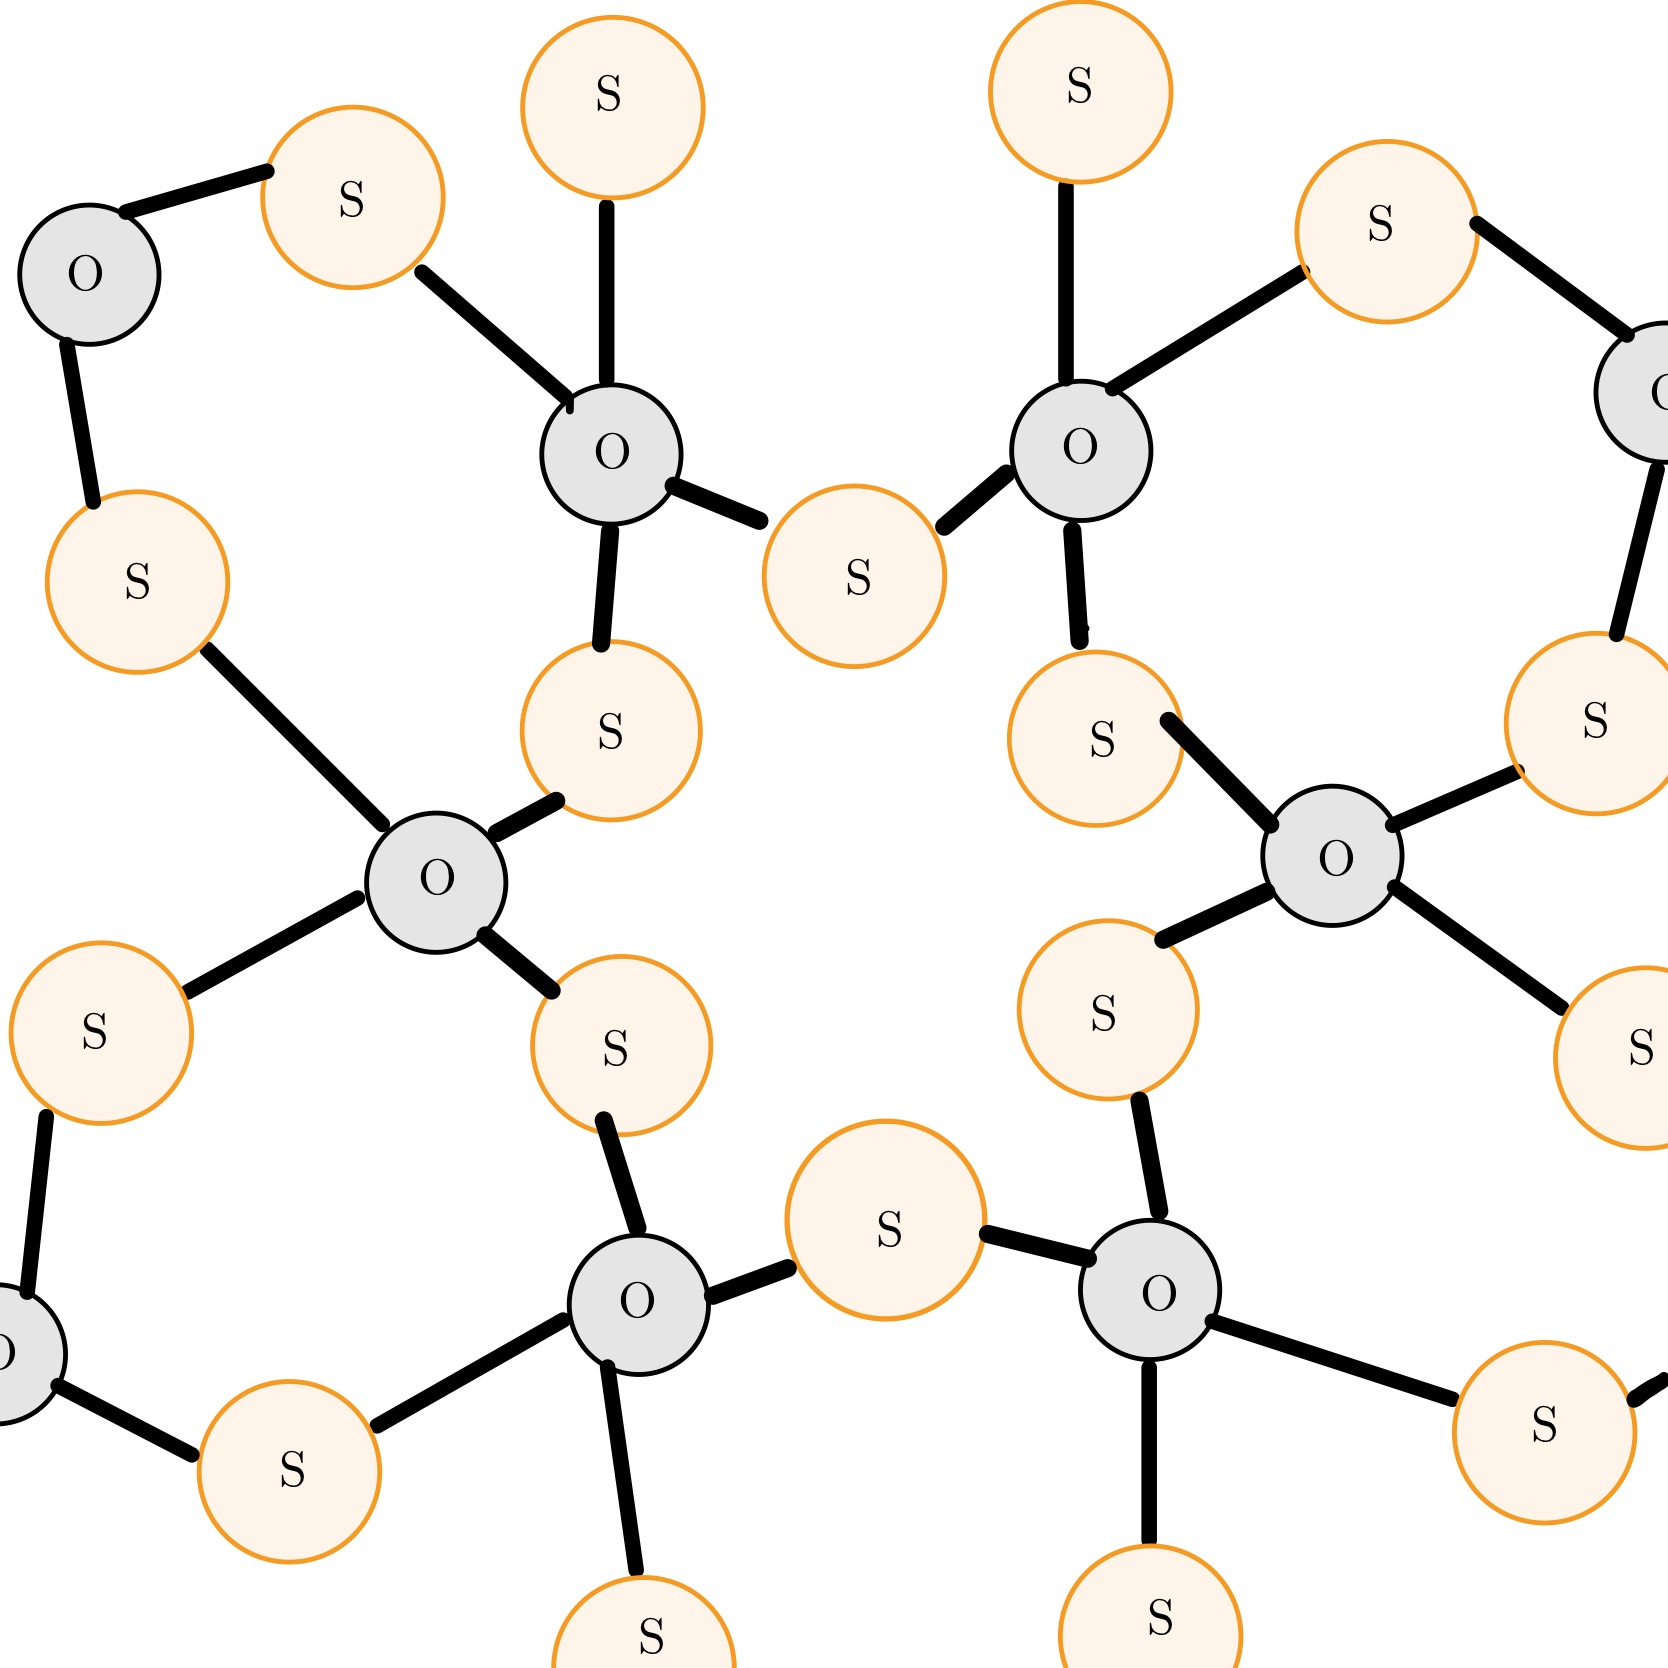
\includegraphics[width=\textwidth]{./Figure_1.jpg}
    \captionof{figure}{Structure of Quartz}
    \label{fig:Structue of Quartz}
\end{minipage}
\begin{minipage}{0.66\textwidth}
    To understand how a piezoelectric element works, one must have a look at the structure of a piezoelectric crystal. Most piezoelectric elements are made from quartz. Quartz is a material composed of silicon-dioxide whose structure can be seen in Figure \ref{fig:Structue of Quartz}. It is made of silicone and oxygen atoms arranged in a hexagonal shape. The silicone atoms are charged positively and the oxygen atoms negatively as the oxygen atom has a higher electronegativity.\cite{Mould2019}\\
\end{minipage}
\begin{minipage}{0.33\textwidth}
    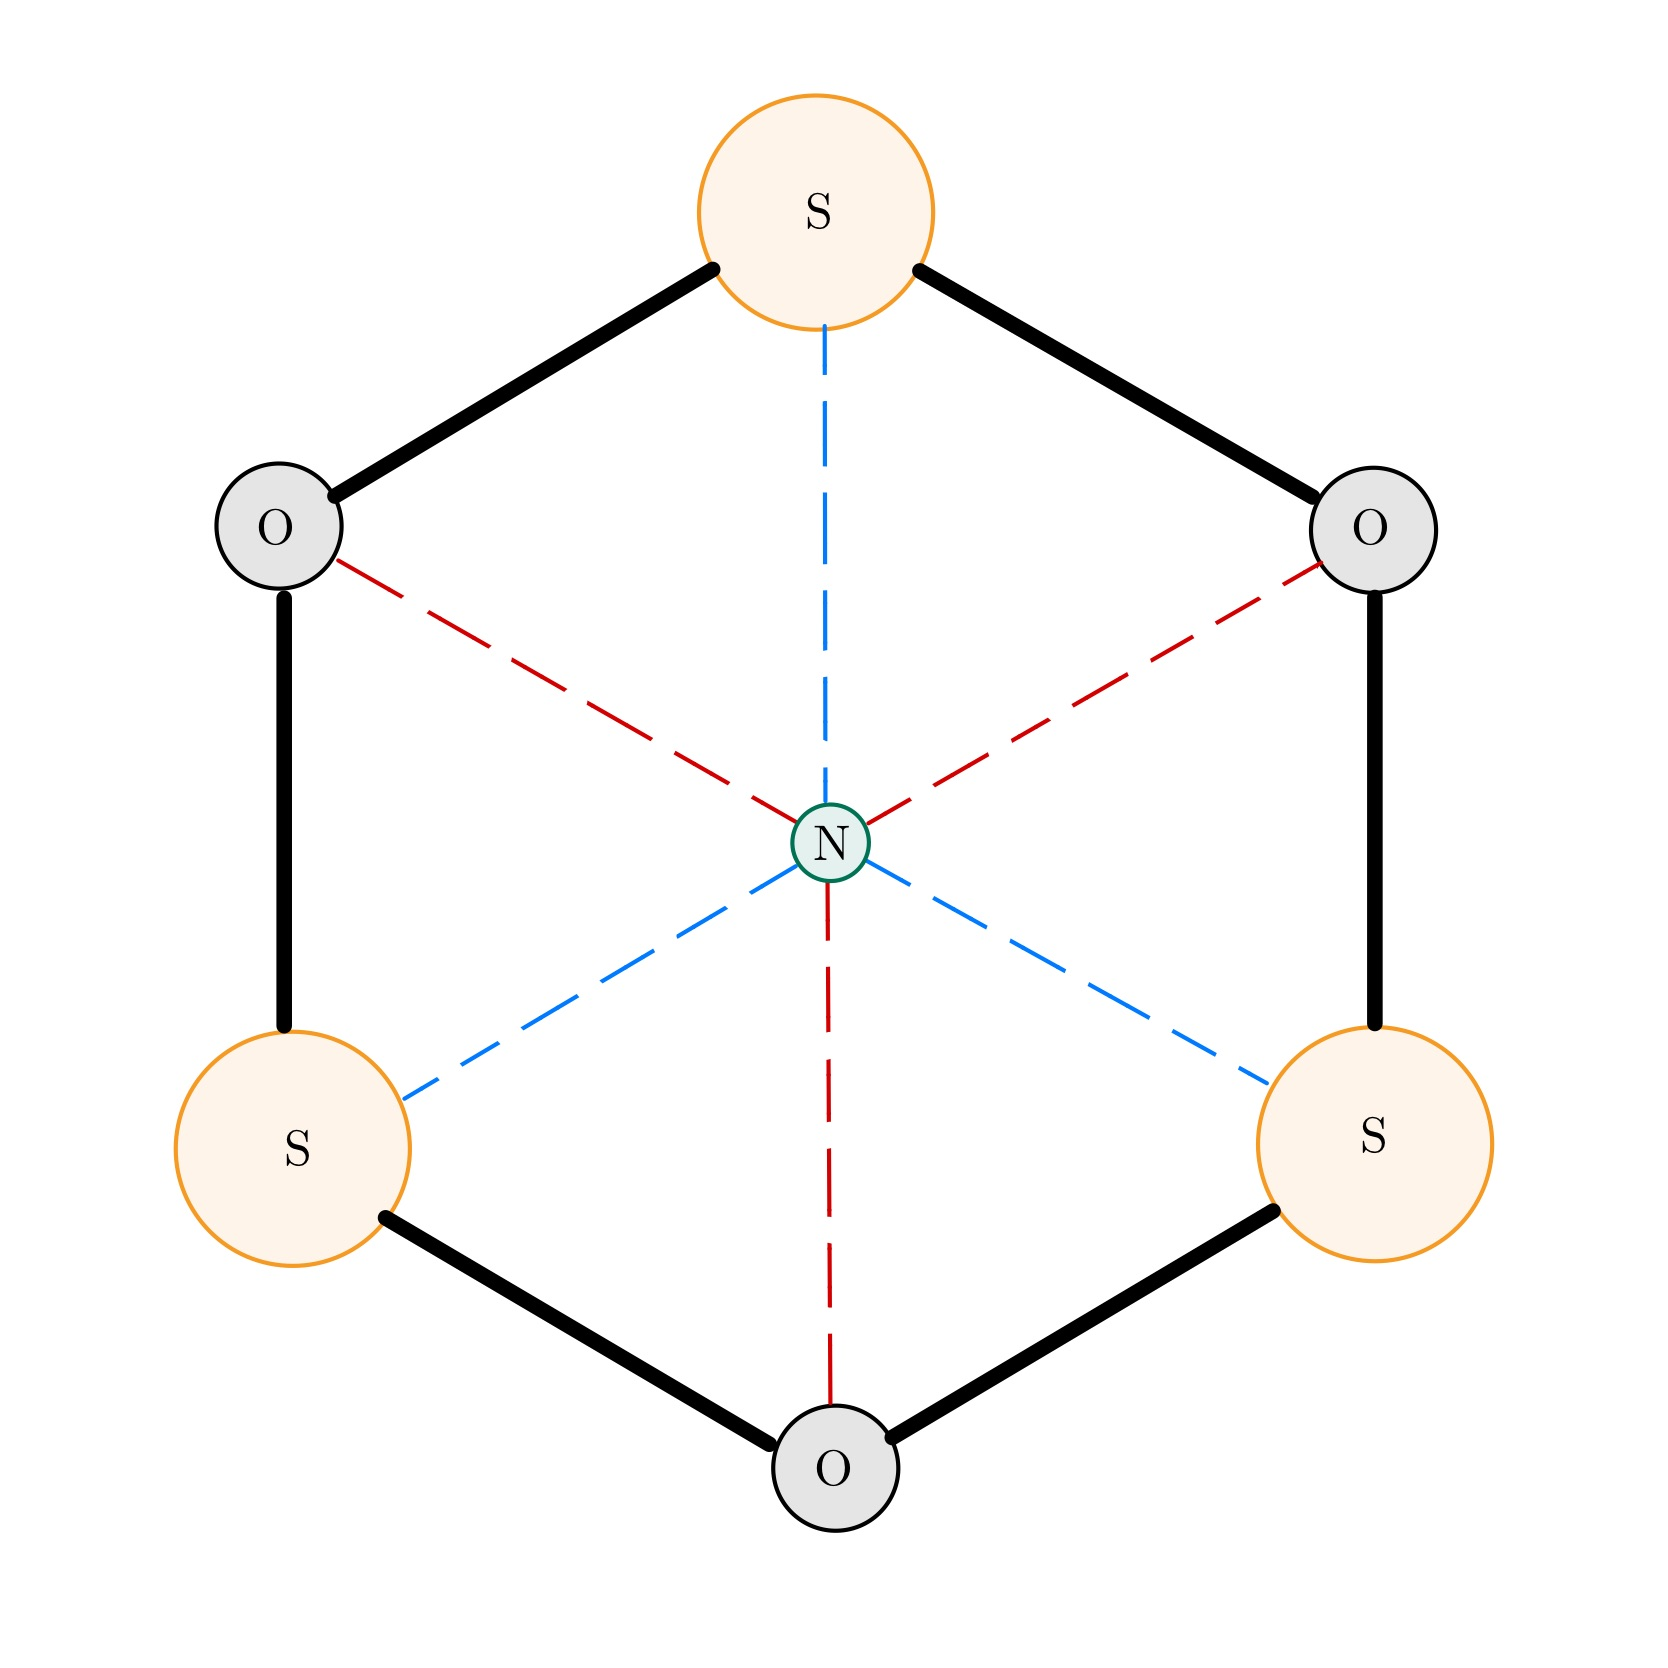
\includegraphics[width=\textwidth]{./Figure_2.jpg}
    \captionof{figure}{Quartzcell without any influence}
    \label{fig:Quartzcell without any influence}
\end{minipage}
\begin{minipage}{0.66\textwidth}
    In the beginning the average position of the charges overlap with each other which is visible in Figure \ref{fig:Quartzcell without any influence}. This means that no electromagnetic field is formed and thus no electric charge flows. However, when mechanical stress is applied onto the crystal the structure is changed.\cite{Mould2019}\\
\end{minipage}
\begin{minipage}{0.33\textwidth}
    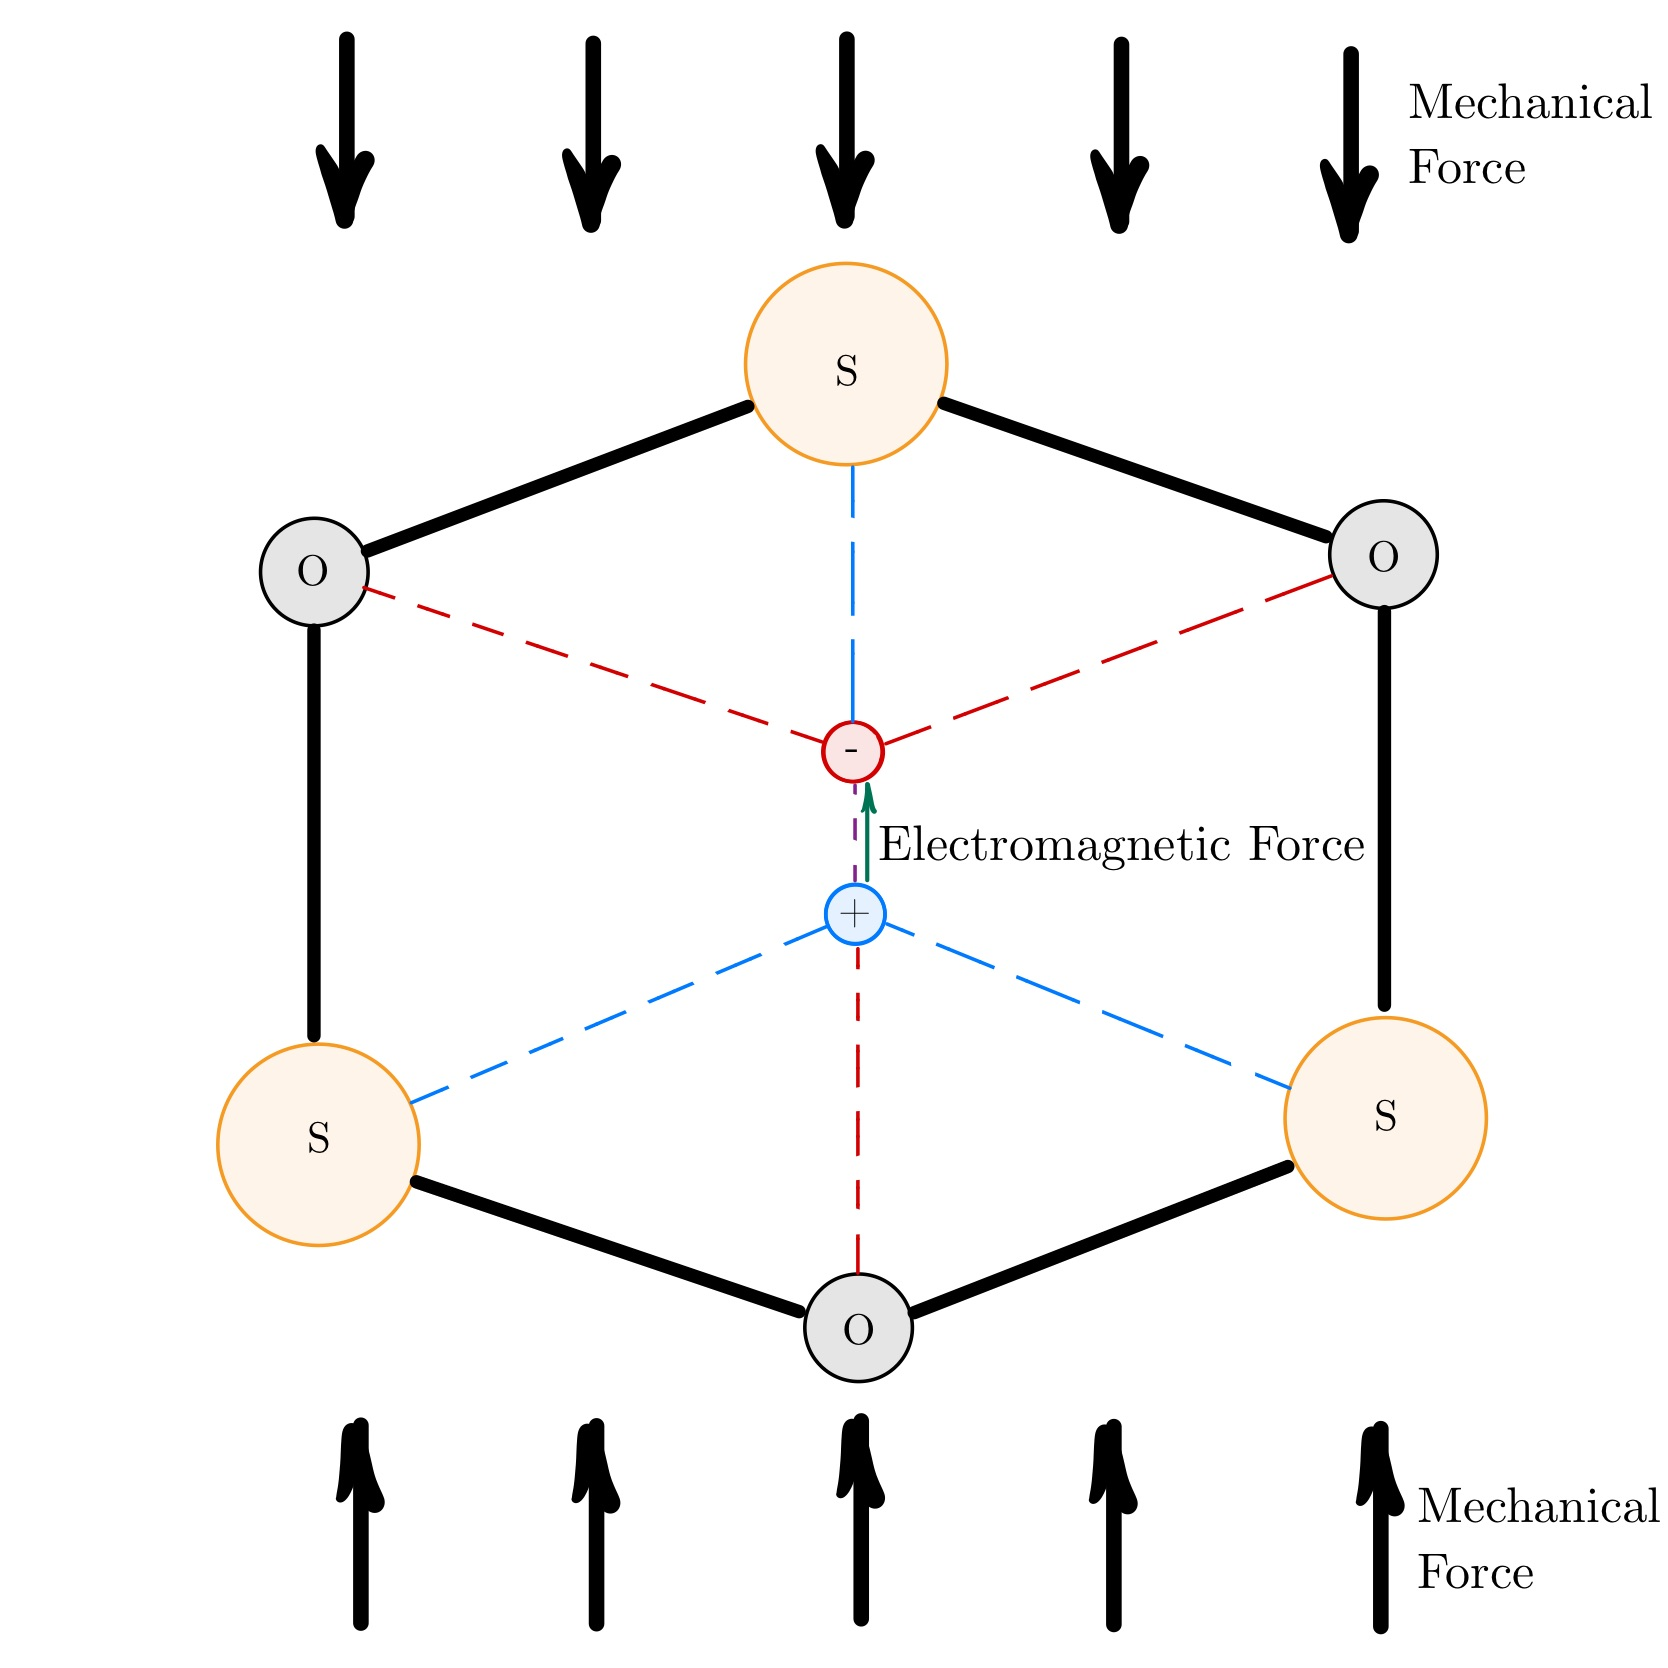
\includegraphics[width=\textwidth]{./Figure_3.jpg}
    \captionof{figure}{Quartzcell compressed}
    \label{fig:Quartzcell compressed}
\end{minipage}
\begin{minipage}{0.66\textwidth}
Mechanical stress can be either in the form of compression or expansion. In case of compression, the average position of the negative charge is moved upwards and the average position of the positive charge is moved downwards (Figure \ref{fig:Quartzcell compressed}) and vice versa when expanded.\cite{Mould2019}\\
\end{minipage}

\vspace{0.5cm}
\noindent In either way, a current can now flow as a positive face and a negative face is created. If a load such as a small LED is connected to the faces, the LED would blink. It is important to note is that the load must be connected correctly. The anode and cathode differ depending on the type of mechanical stress.\\
\begin{minipage}{0.33\textwidth}
    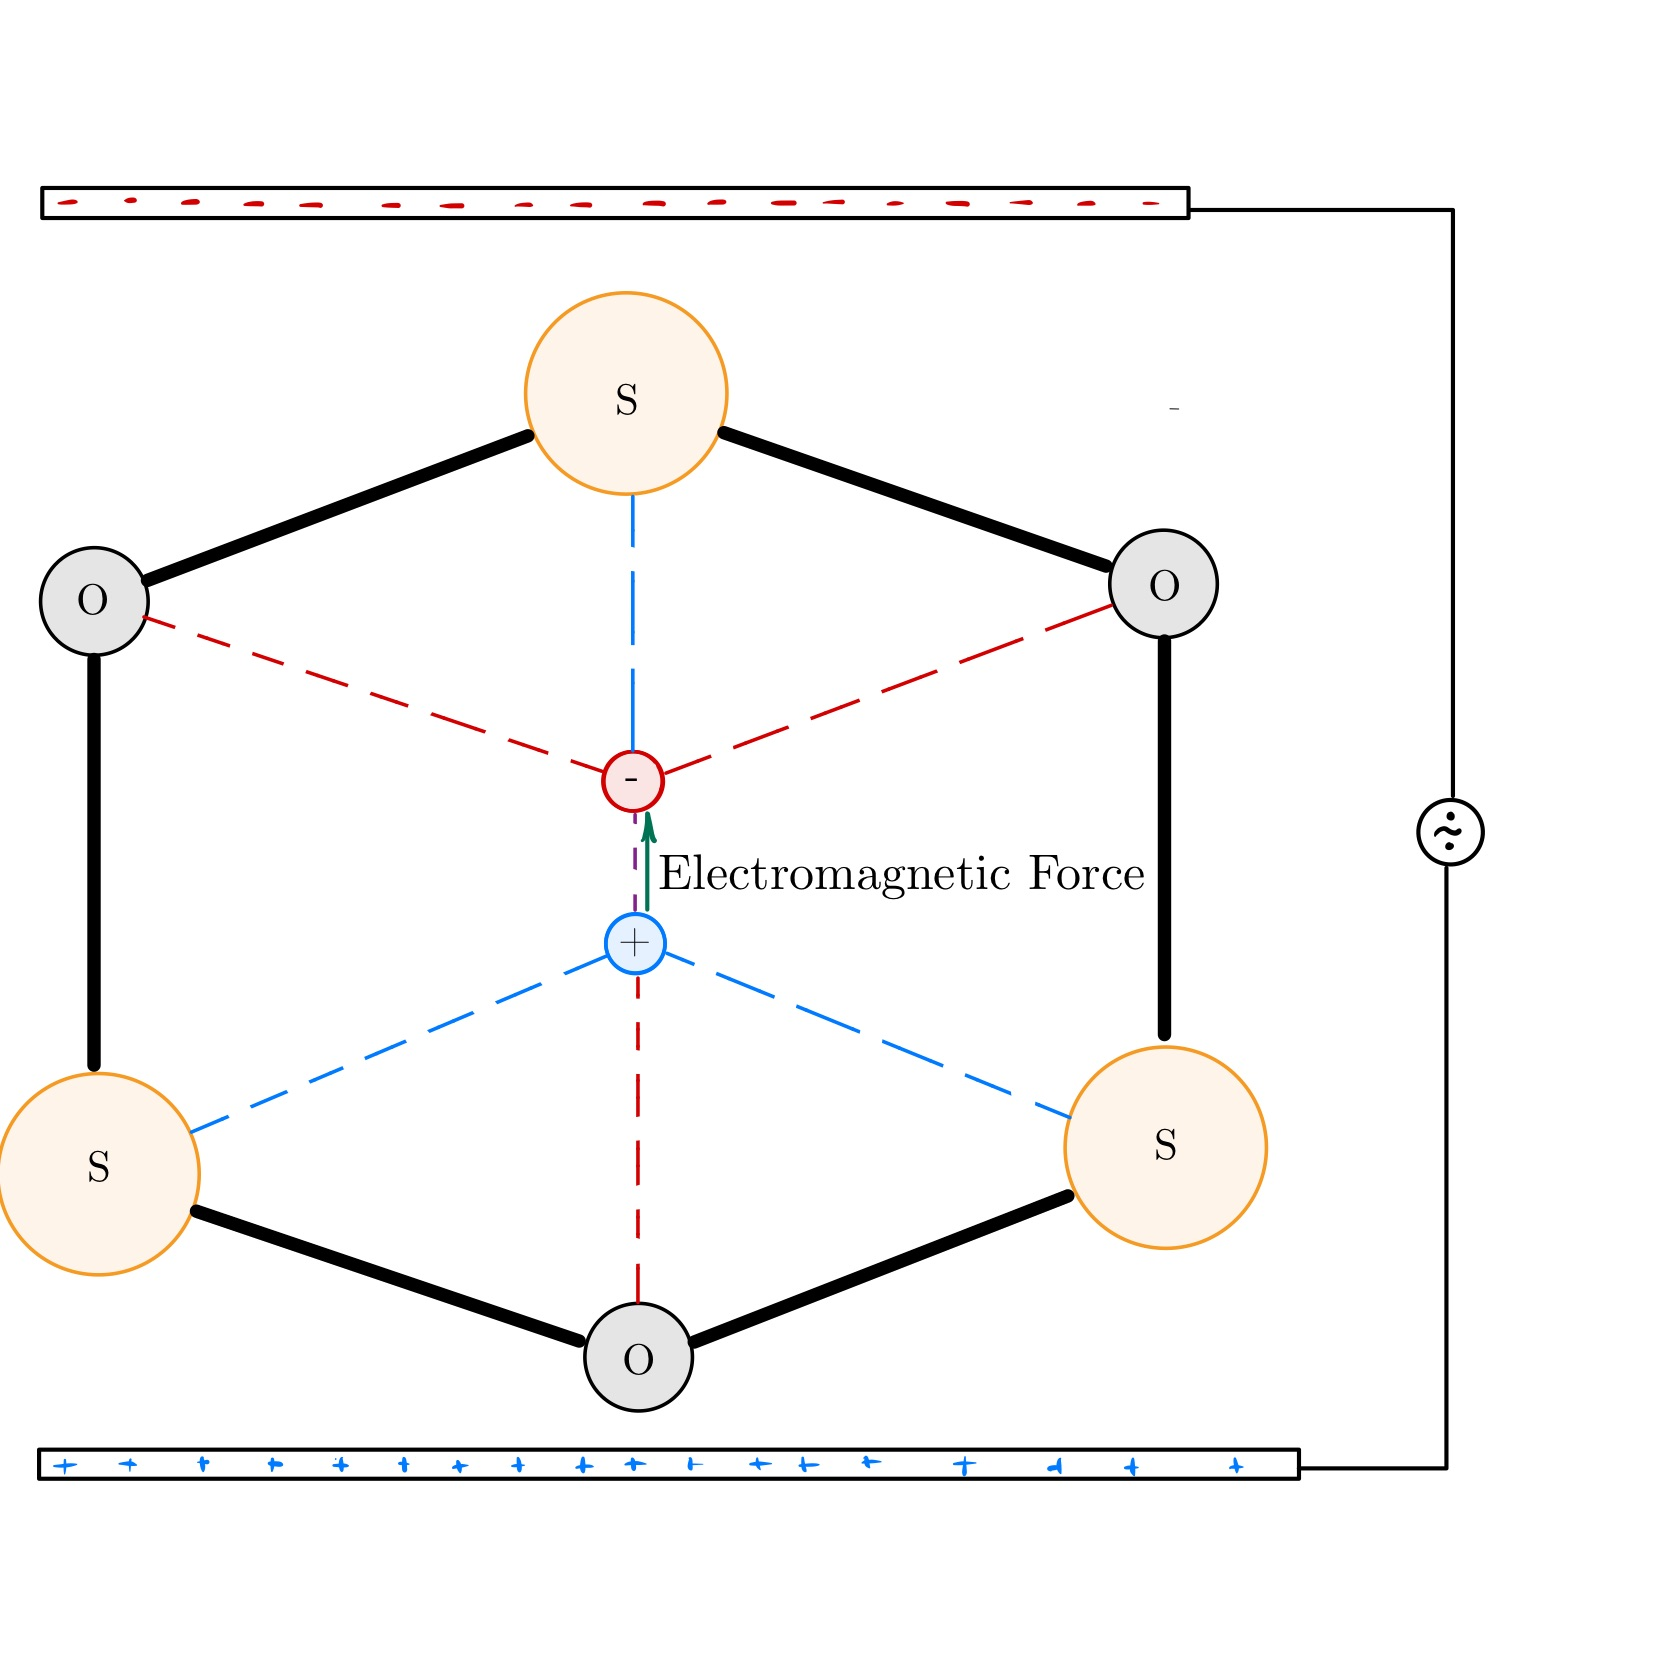
\includegraphics[width=\textwidth]{./Figure_4.jpg}
    \captionof{figure}{Quartzcell charged with a voltage}
    \label{fig:Quartzcell charged with a voltage}
\end{minipage}
\begin{minipage}{0.66\textwidth}
    Besides the mechanical stress, a voltage can be applied onto the crystal. This is refered to as the reciprocal piezoelectric effect. When the cathode and anode are positioned like in  Figure \ref{fig:Quartzcell charged with a voltage} the crystal will be compressed since the anode repels the negatively charged oxygen and the cathode repels the positively charged silicone and vice versa.\cite{Elprocus2023}\\
\end{minipage}
\\
 
\subsection{Formula}

To have a comparison with the measured voltage, the voltage output has to be calculated. The formula for the voltage output of a piezoelectric element can be calculated by simplifying the voltage output of a capacitor since the piezoelectric element is a capacitor.\cite{F3lixTutorial2023}\\
Before going through the process of simplifying the formula, two piezoelectric constants must be defined. There are many, however, only the electromechanical coupling factor and the piezoelectric voltage constant will be defined as only these constants will be used. The electromechanical coupling factor $d$ is defined as the effectiveness with which a piezoelectric element converts mechanical energy into electrical energy and vice versa. The piezoelectric voltage constant $g$ is defined as the electric field generated by a piezoelectric element per unit stress applied. The constants differ depending on the direction of mechanical stress or the electrical field.\cite{F3lixTutorial2023}\\
\begin{minipage}{0.33\textwidth}
    \vspace{0.5cm}
    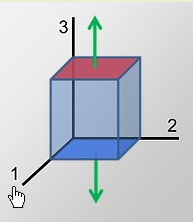
\includegraphics[width=\textwidth]{./Figure_5.jpg}
    \captionof{figure}{Expansion Mode of the Piezoelectric Element \cite{F3lixTutorial2023}}
    \label{fig:Expansion Mode of the Piezoelectric Element}
\end{minipage}
\begin{minipage}{0.66\textwidth}
    The constants are marked with numbers. These numbers correspond to the direction of mechanical stress and the polarization which is depicted in Table \ref{Tab:Piezoelectric Constants} and Figure \ref{fig:Expansion Mode of the Piezoelectric Element}. In our case $g_{33}$ and $d_{33}$ will be used since the force acting on the crystal is from direction 3 and the polarization occurs in direction 3.\cite{F3lixTutorial2023}\\ 
\end{minipage}
\begin{minipage}{0.5\textwidth}
    \center
        \begin{tabular}{|c|c|c|c|}
            \hline
            & PZT-5H & PZT-5A & PZT-5J \\
            \hline
            \hline
            $d_{31}$ & -320 & -190 & -270 \\
            \hline
            $d_{33}$ & 650 & 390 & 485 \\
            \hline
            $d_{15}$ & 1000 & 460 & 850 \\
            \hline
            $g_{31}$ & -9.5 & -11.3 & -11.5 \\
            \hline
            $g_{33}$ & 19.0 & 23.2 & 21.3 \\
            \hline
            $g_{15}$ & 35.3 & 32.4 & 32.6 \\
            \hline
        \end{tabular}
        \captionof{table}{Piezoelectric Constants \cite{Carter2023}}
        \label{Tab:Piezoelectric Constants}
\end{minipage}
\begin{minipage}{0.5\textwidth}
    From Table \ref{Tab:Piezoelectric Constants}, one can see that the constant also depends on the type of piezoelectric material. There are three types of piezoelectric materials which are commonly used. The piezoelectric material used in this experiment is of type PZT-5J since the material was made from ceramic and the cathode was made from silver. This ensures that the piezoelectric element performs well under the specific stress and voltage. Depending on the direction, the type of piezo is chosen to maximise the energy outcome. However, most piezos are of type PZT-5J since they are considered to be an allrounder for any case of stress or voltage. \cite{Carter2023}\\
\end{minipage}
Since the piezoelectric element is a capacitor, the formula $U=\frac{Q}{C}$ can be used where $U$ is the voltage, $Q$ is the charge and $C$ is the capacity. From there the formula $\epsilon \cdot \frac{A}{t}$ is inserted where $\epsilon$ is the permitivity, $A$ is the surface area where the mechanical stress is applied on and $t$ is the thickness of the piezoelectric element. Furthermore, the formula $d \cdot F$ can be inserted for $Q$ where $F$ is the force applied onto the piezoelectric element and $d$ is the effeciveness with wwhich a piezoelectric element converts mechanical energy into electrical energy and vice versa. Once all equations are inserted, $U=\frac{d \cdot F \cdot t}{\epsilon \cdot A}$ where $\frac{d}{\epsilon}$ can be replaced with $g$. This results in the formula $U = g \cdot \frac{F \cdot t}{A}$ for the Voltage output of the piezoelectric element. \cite{F3lixTutorial2023}
$$
U = \frac{Q}{C} \quad \text{ where } C = \epsilon \cdot \frac{A}{t} \text{ and } Q = d \cdot F
$$
$$
U = \frac{d \cdot F \cdot t}{\epsilon \cdot A} \text{ where } g = \frac{d}{\epsilon}
$$
$$
U = g \cdot \frac{F \cdot t}{A}
$$
For the energy emitted by the piezoelectric element, on can use the formula for the energy of a spring since the compression and expansion is similar to a spring. Hence, the formula $E = \frac 1 2 \cdot F \cdot x$ applies where $E$ is the energy, $F$ is the force applied onto the piezoelectric element, and $x$ is the displacement of the element. Since $x$ is not known, it can be replaced by $\frac{F}{k}$ where $k$ is the sping constant of the piezoelectric element. This leads the formula $E = \frac{1}{2} \cdot F \cdot \frac F k$ for the energy outputted by the piezoelectric element.
$$
E = \frac{1}{2} \cdot F \cdot x \text{ where } x = \frac{F}{k}
$$
$$
E = \frac{1}{2} \cdot F \cdot \frac{F}{k}
$$ %       \
\chapter{Experiment}

\section{Setup}

\begin{minipage}{0.33\textwidth}
    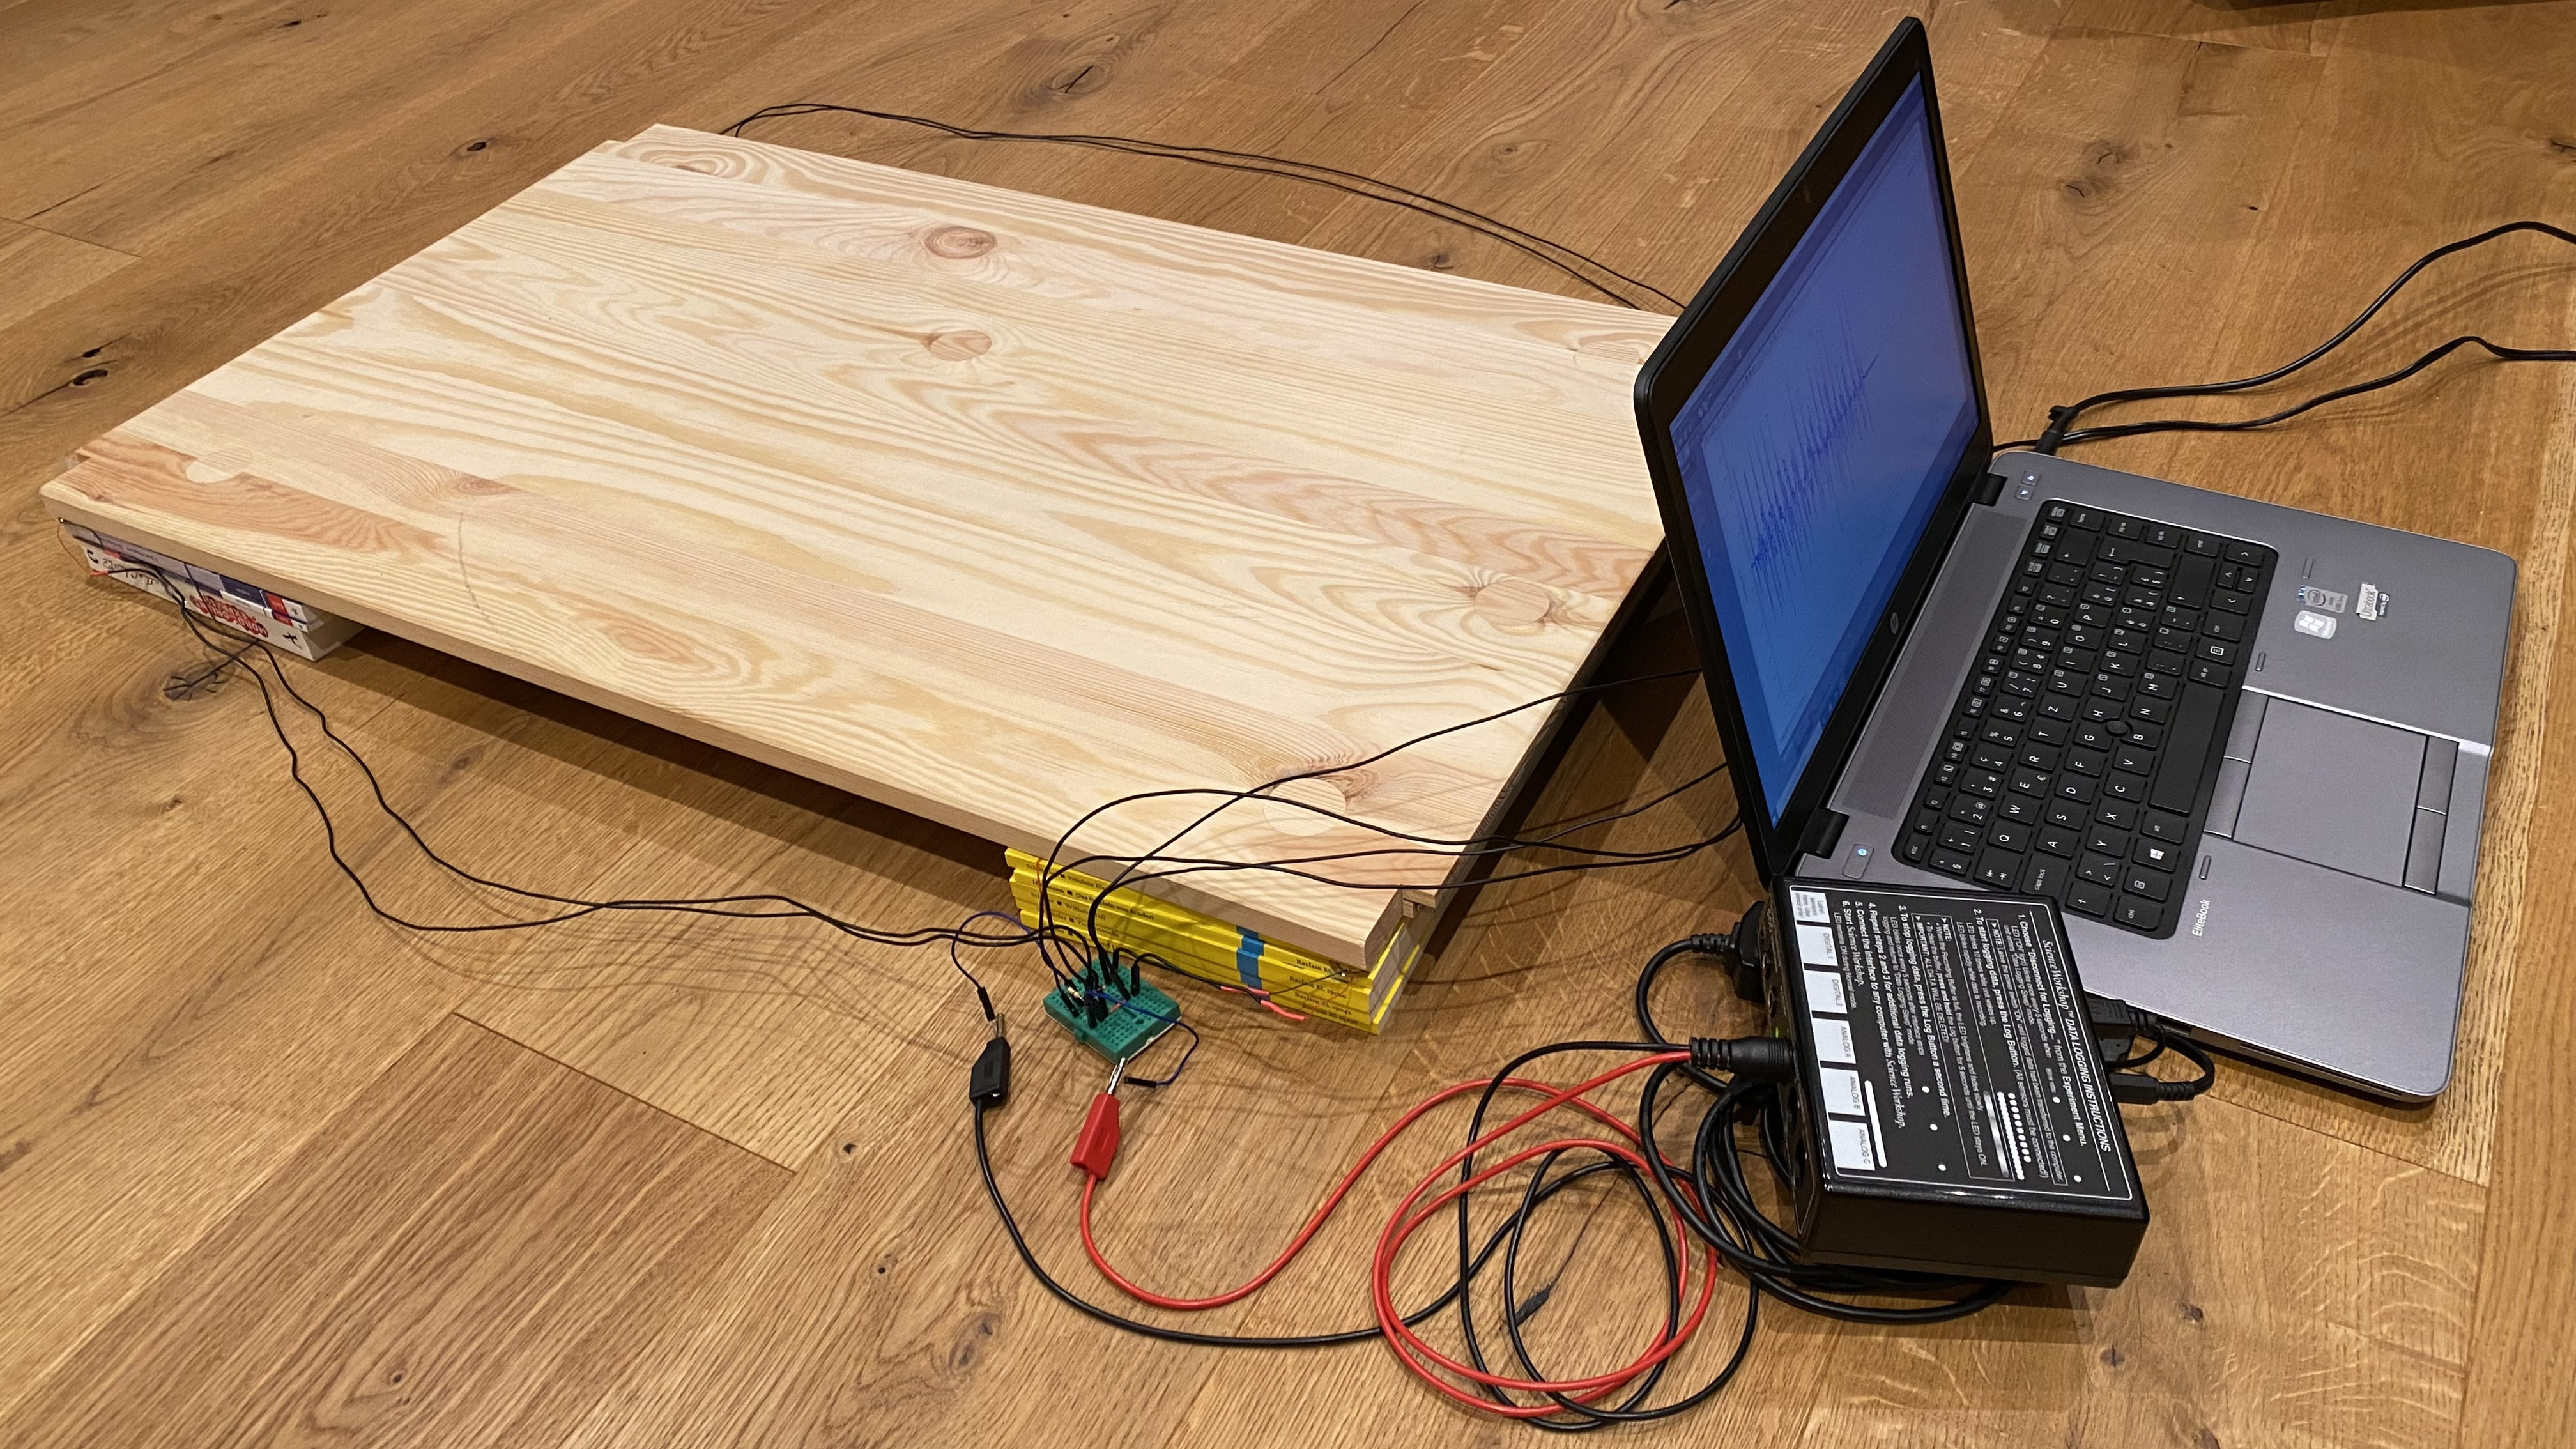
\includegraphics[width=\textwidth]{./Figure_6.jpg}
    \captionof{figure}{Experiment}
    \label{fig:Experiment}
\end{minipage}
\begin{minipage}{0.66\textwidth}
    For the experiment four piezoelectric elements were placed under the corners of a wooden board of dimensions $0.8 \times 0.4 \times 0.02$ m. (Figure \ref{fig:Experiment}) These were then connected to a brad board parallel to a $470k\Omega$ resistor. A voltmeter was connected to the resistor and measured the voltage output while a person was jumping on the wooden board from a height of 20 cm $\pm 1$ cm.\\
\end{minipage}
\begin{minipage}{0.33\textwidth}
    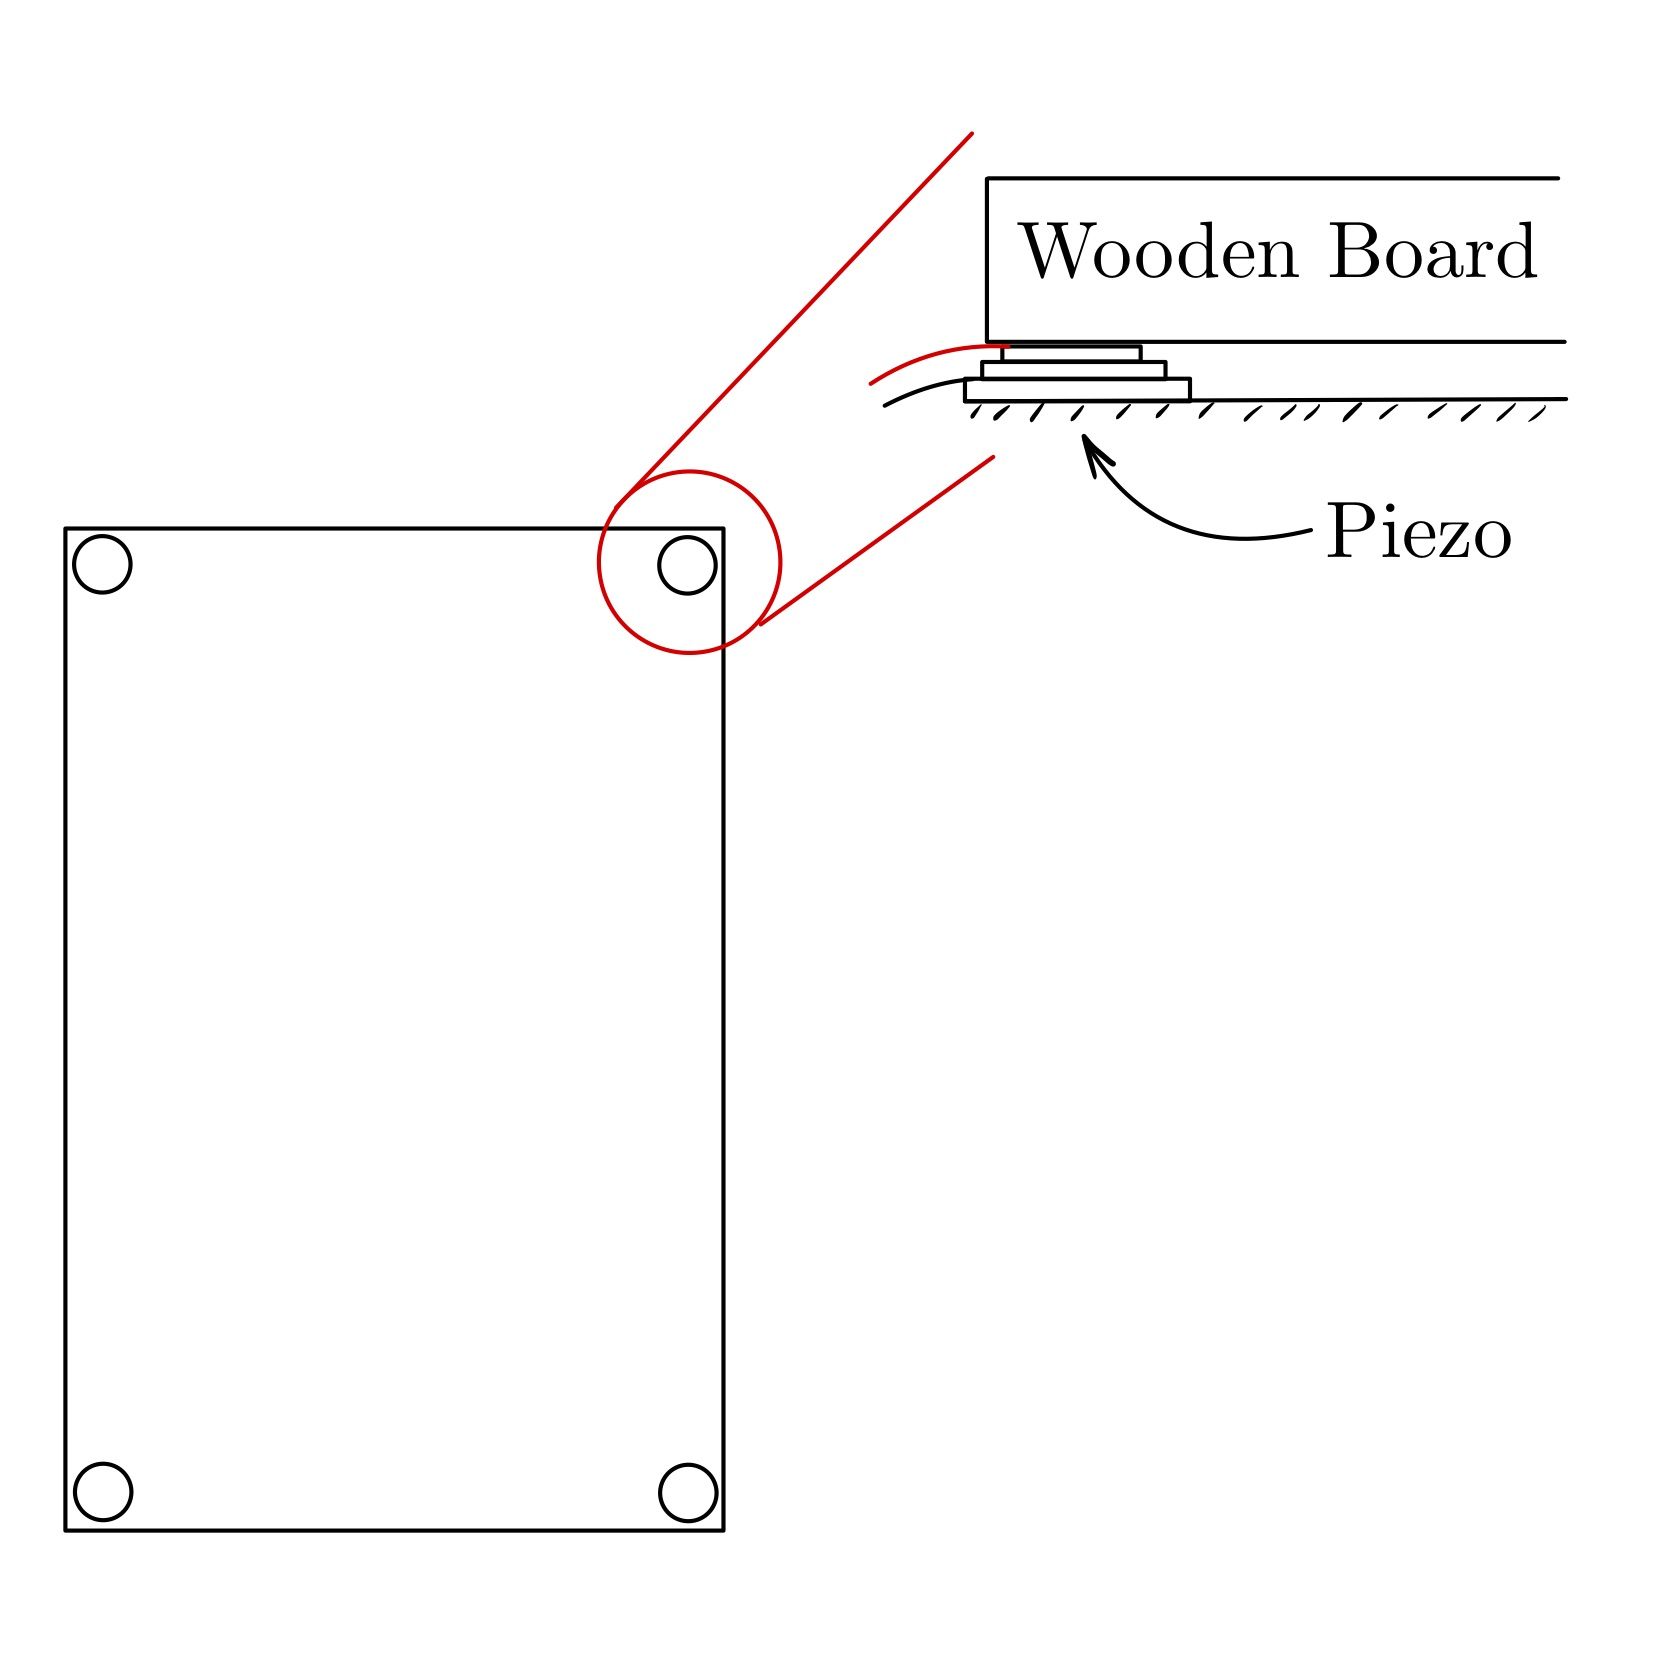
\includegraphics[width=\textwidth]{./Figure_7.jpg}
    \captionof{figure}{Wooden board with piezoelectric elements}
    \label{fig:Wooden board with piezoelectric elements}
\end{minipage}
\begin{minipage}{0.66\textwidth}
    To get an ideal result, the board must be elevated as in Figure \ref{fig:Wooden board with piezoelectric elements}. This ensures an ideal result for the experiment since all the force will be applied onto the four piezo electric elements.\\
\end{minipage}
\begin{minipage}{0.33\textwidth}
    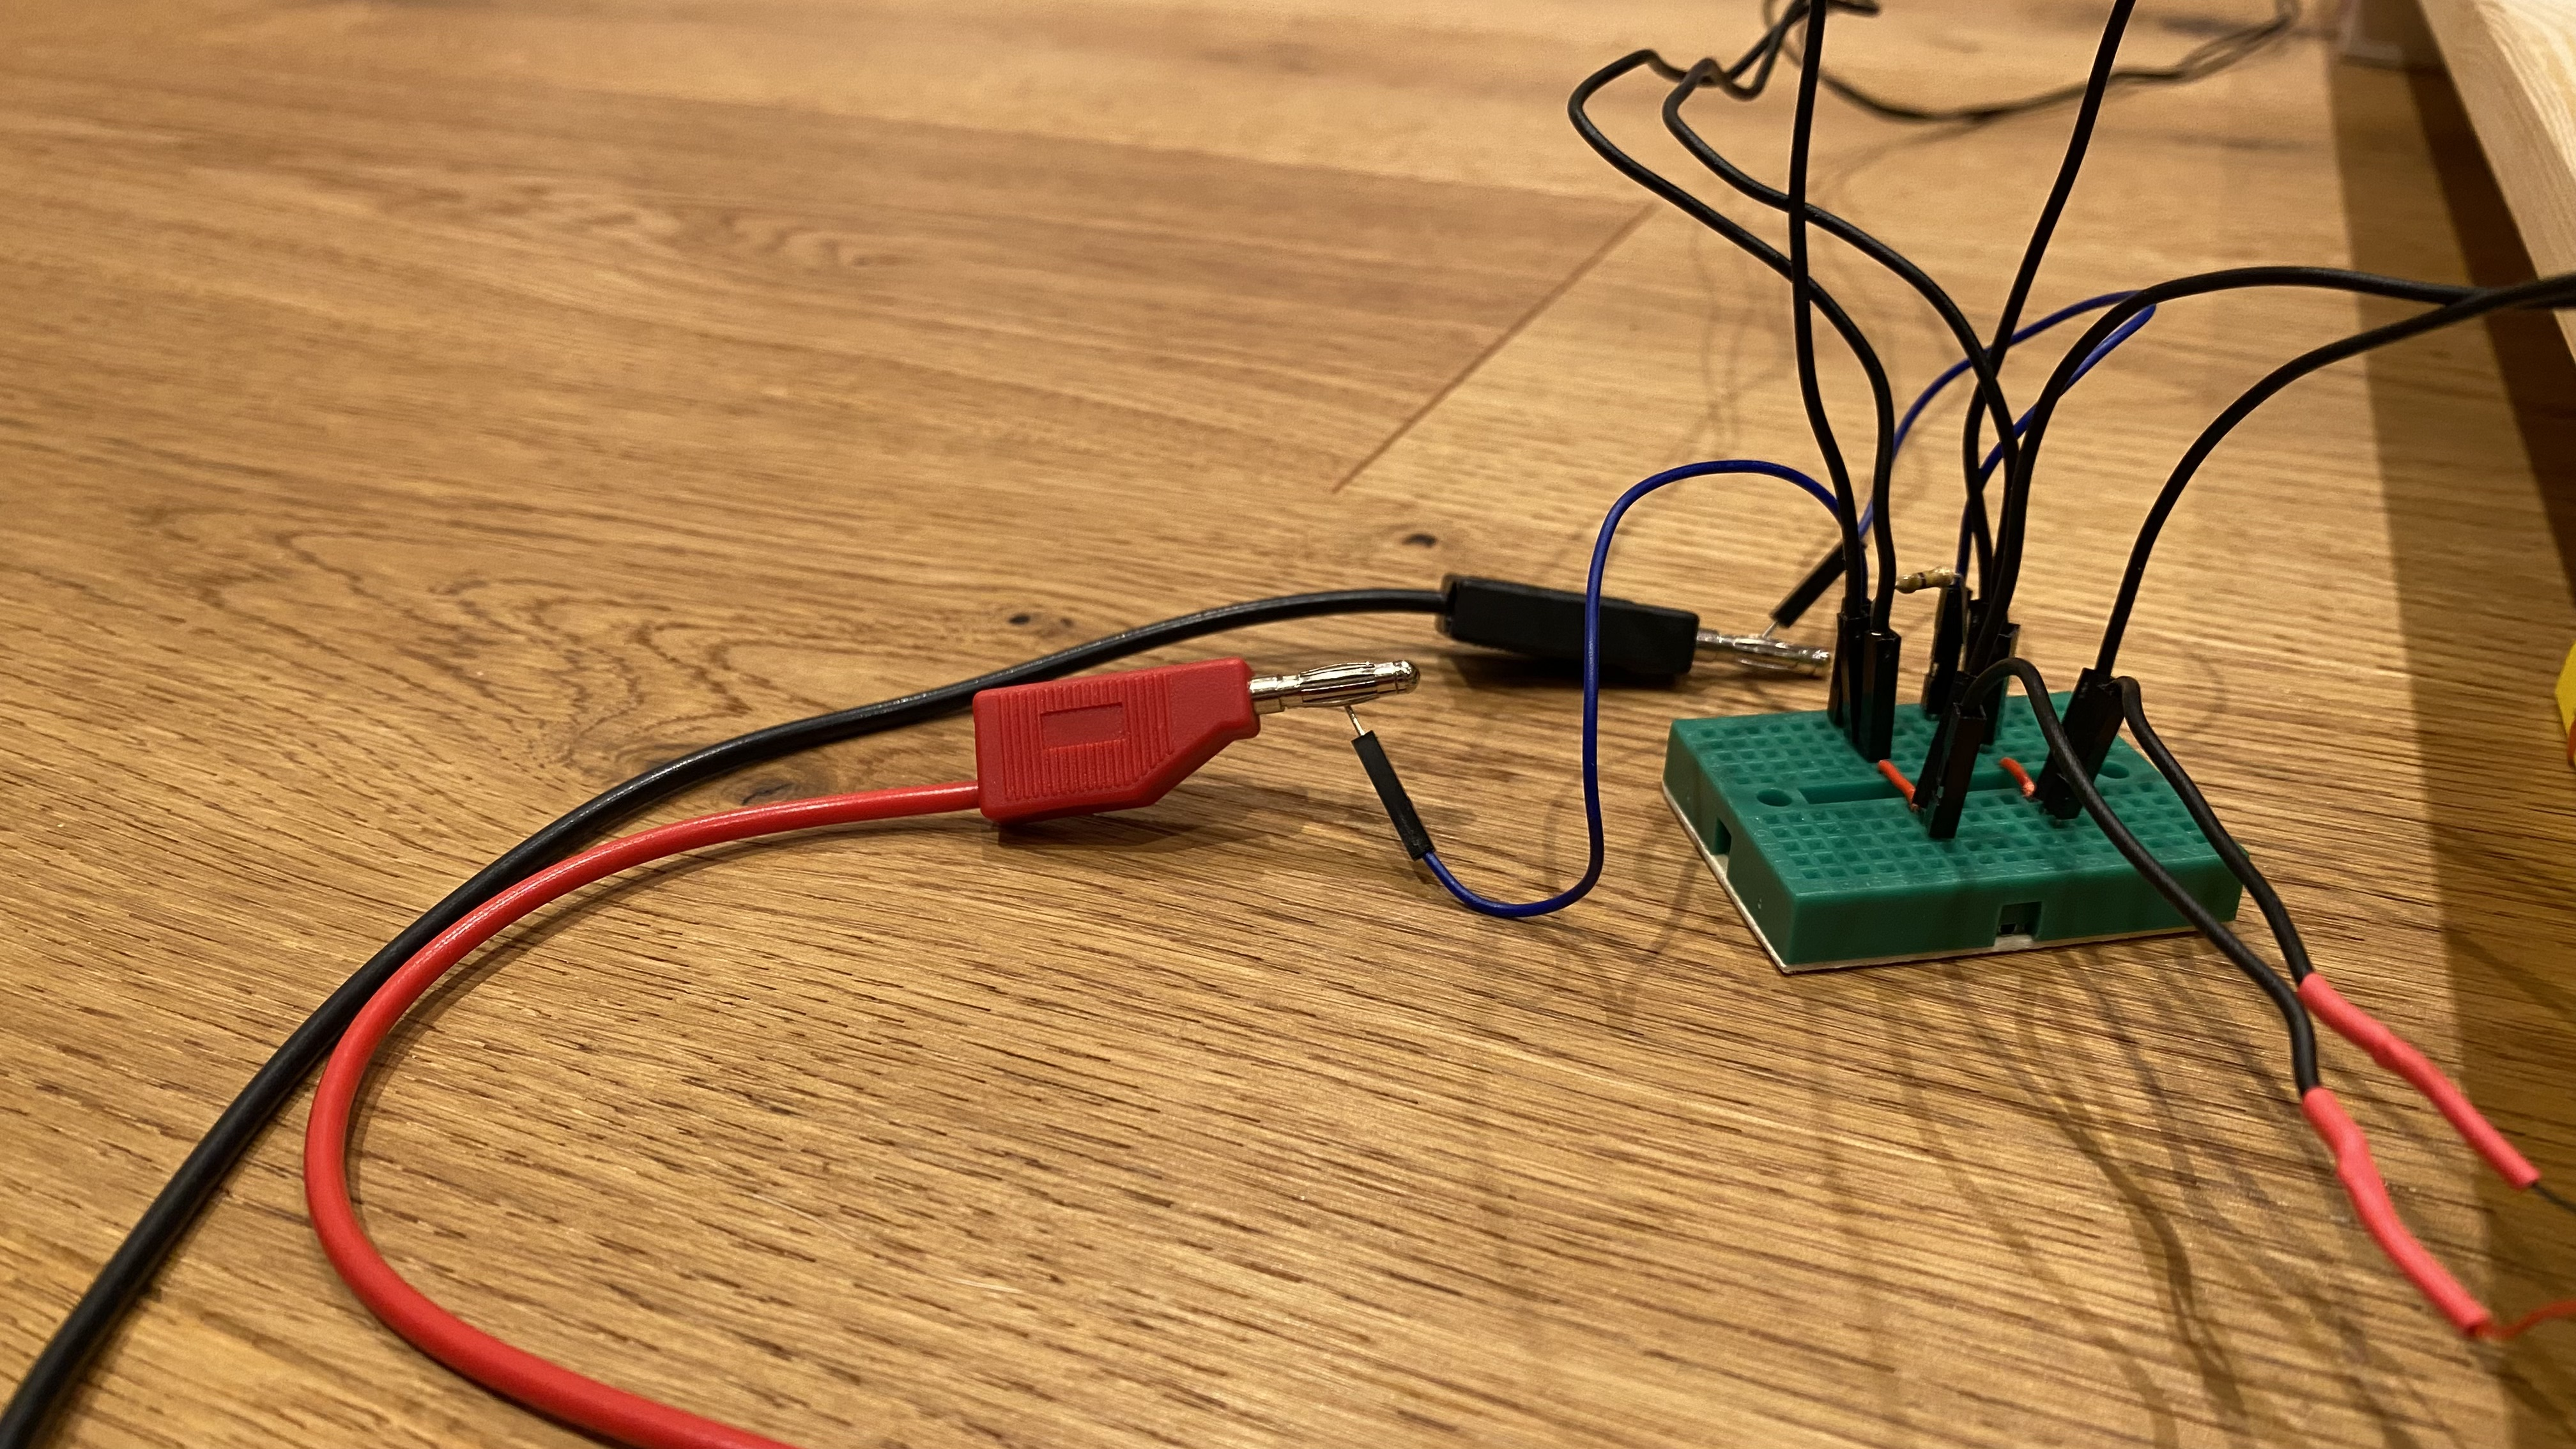
\includegraphics[width=\textwidth]{./Figure_8.jpg}
    \captionof{figure}{Piezoelectric Elements connected in parallel}
    \label{fig:Piezoelectric Elements connected in parallel}
\end{minipage}
\begin{minipage}{0.33\textwidth}
    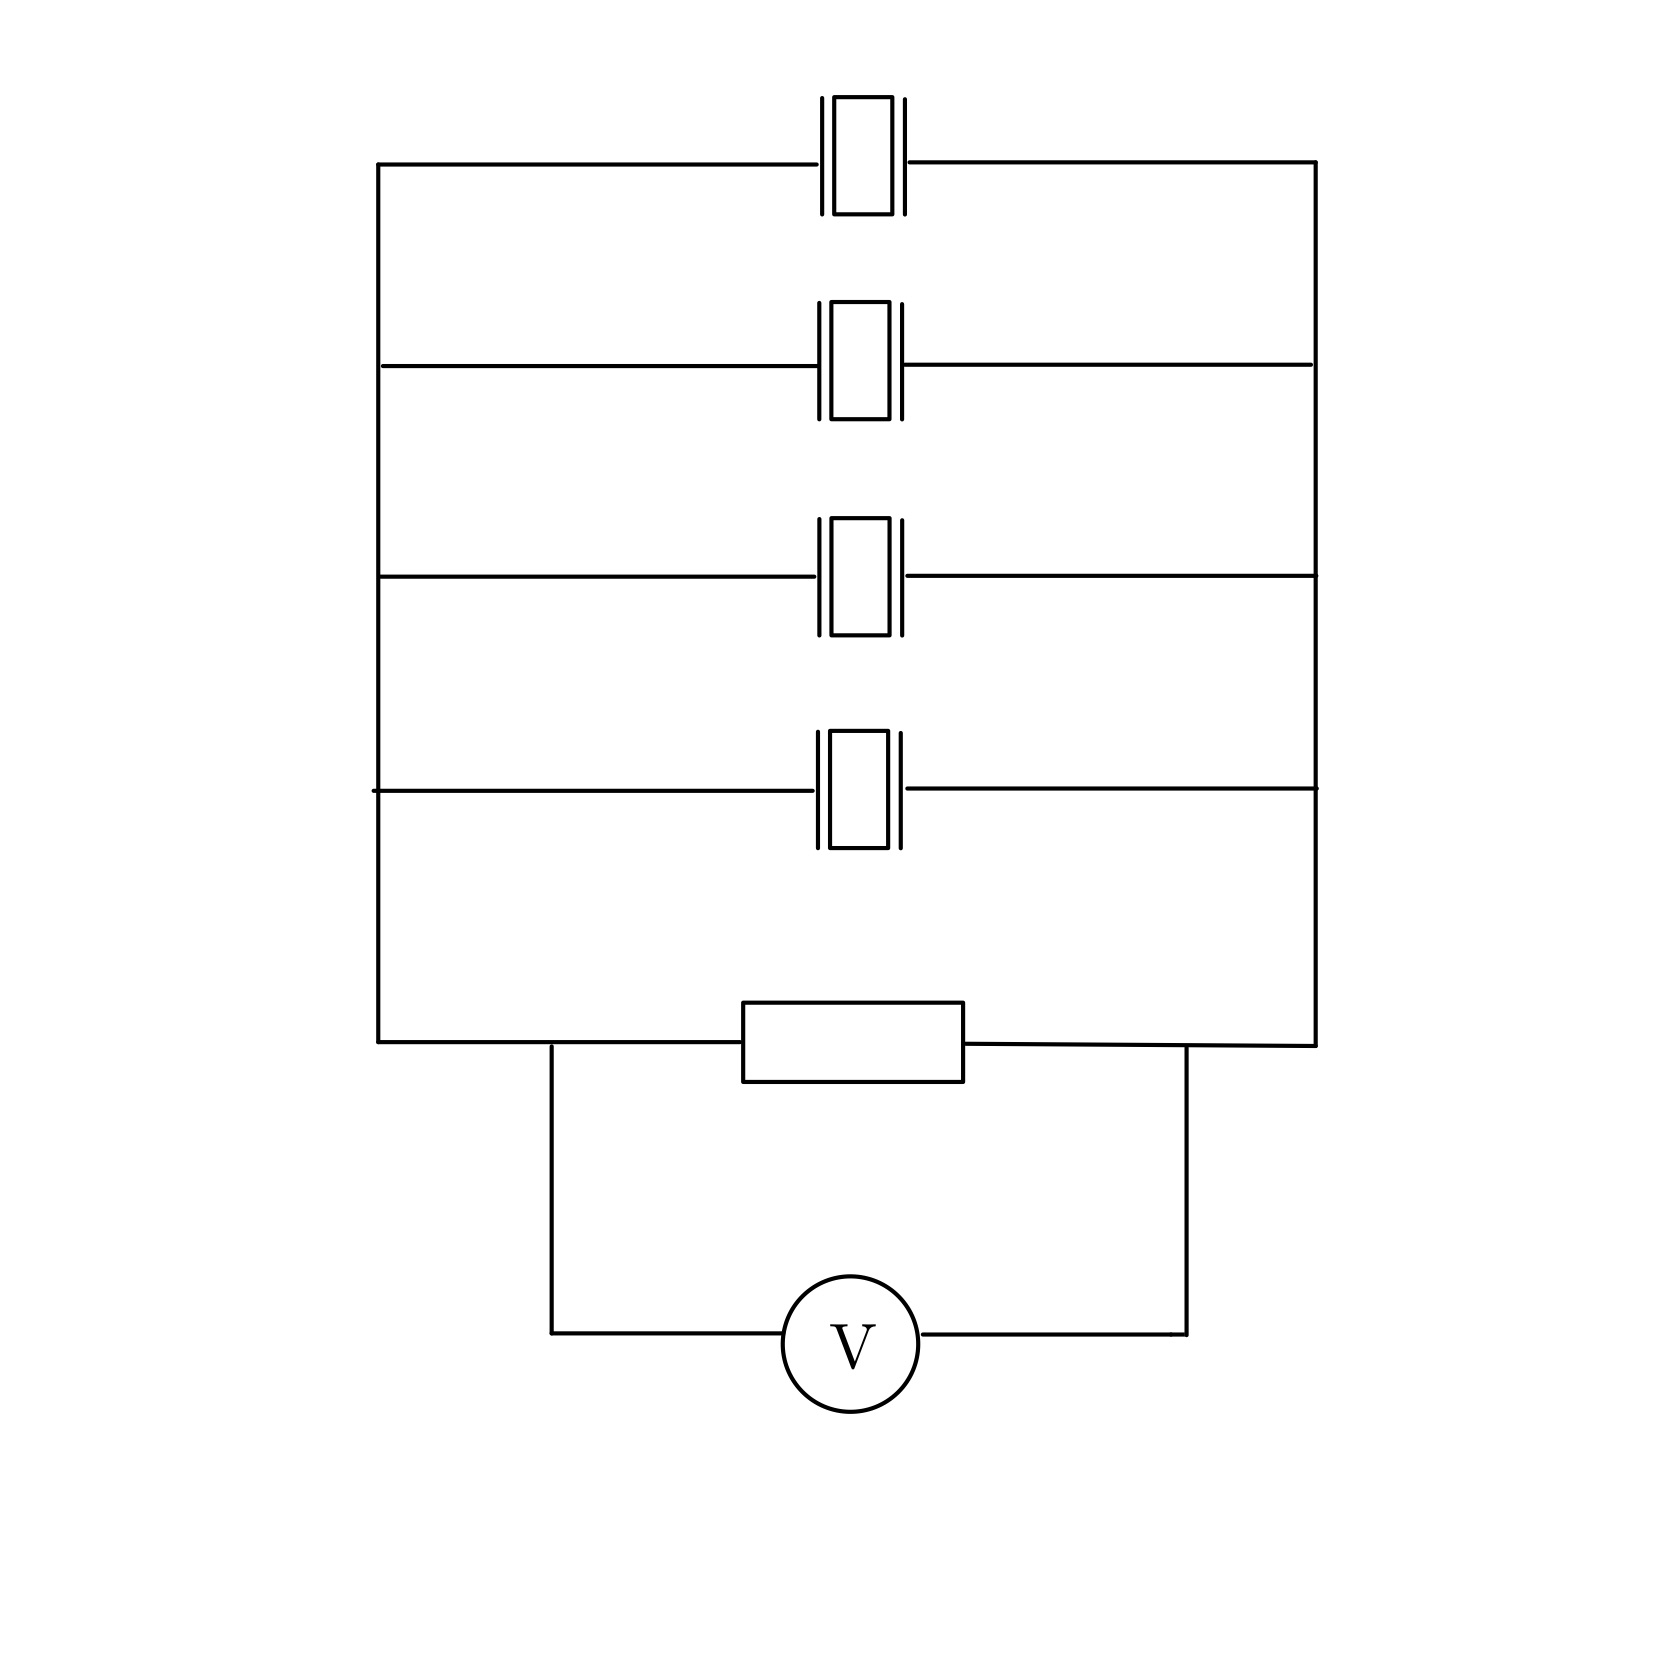
\includegraphics[width=\textwidth]{./Figure_9.jpg}
    \captionof{figure}{Circuit Diagram}
    \label{fig:Circuit Diagram}
\end{minipage}
\begin{minipage}{0.33\textwidth}
    The piezoelectric elements were connected in parallel in addition with a $470k\Omega$ resistor. As represented in Figure \ref{fig:Piezoelectric Elements connected in parallel} and \ref{fig:Circuit Diagram} the voltmeter was then parallel connected to the resistor.\\
\end{minipage}
\begin{minipage}{0.33\textwidth}
    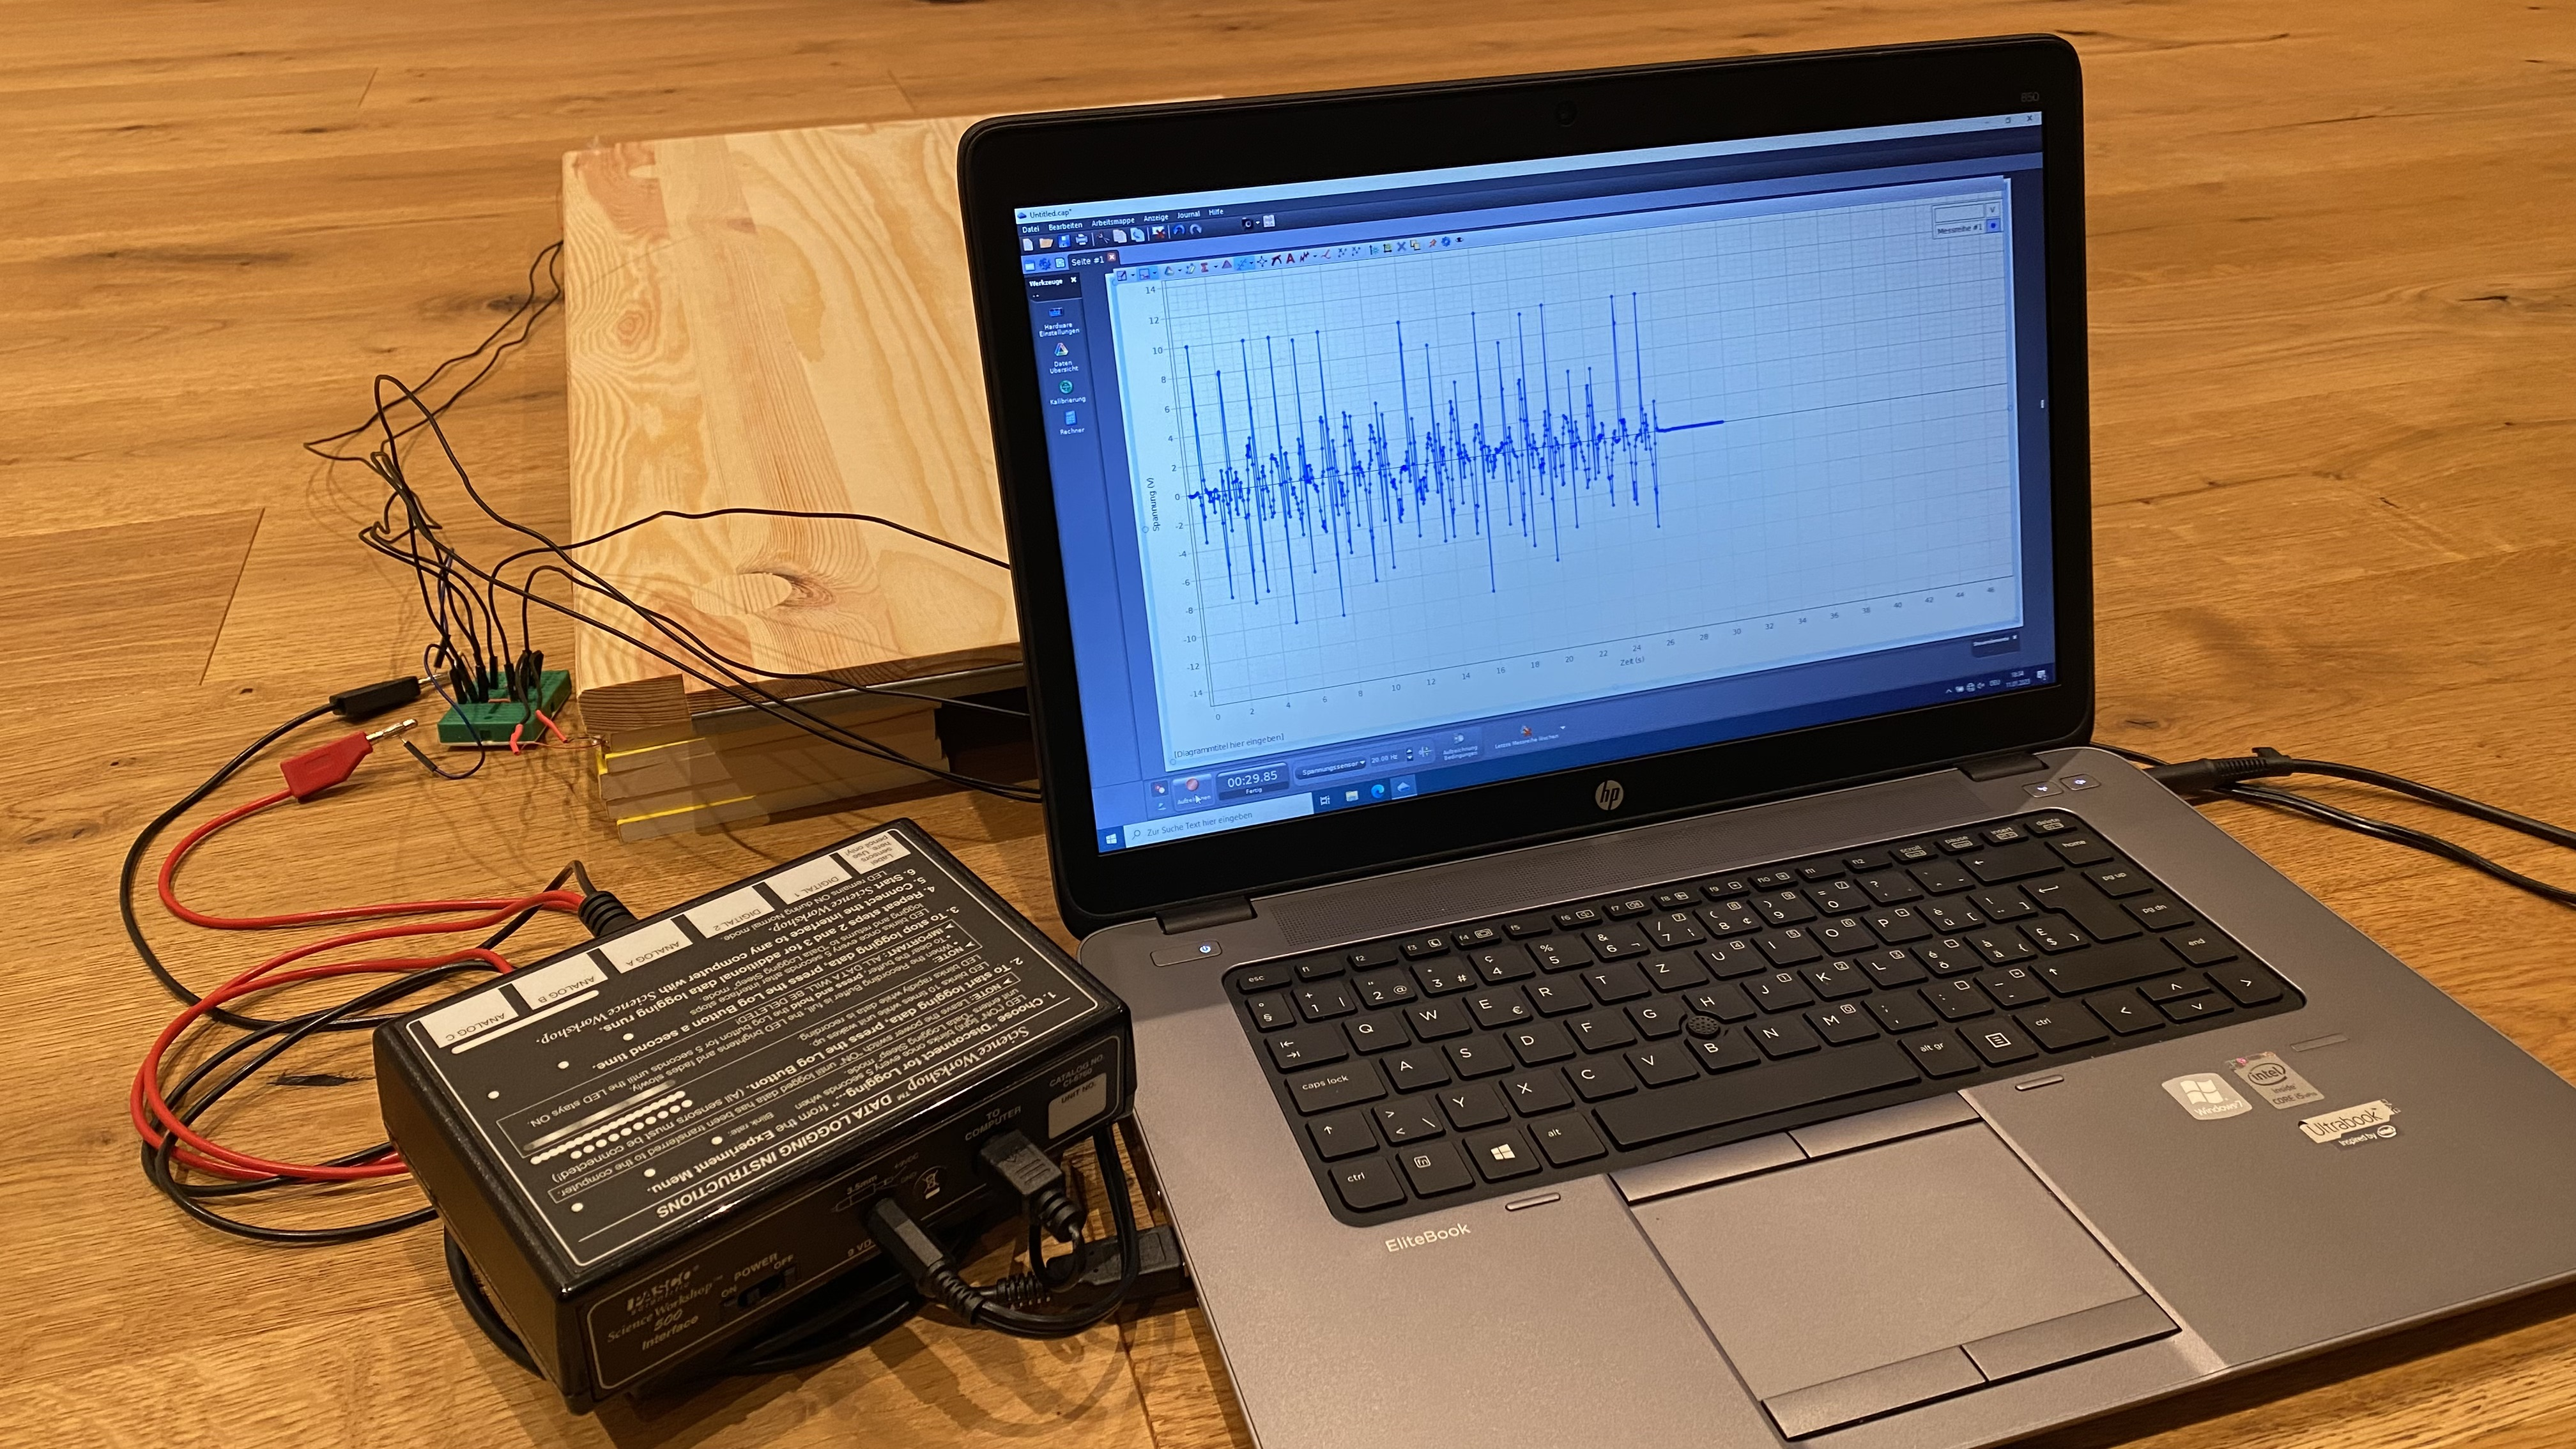
\includegraphics[width=\textwidth]{./Figure_10.jpg}
    \captionof{figure}{Laptop and Pasco Interface 500}
    \label{fig:Laptop and Pasco Interface 500}
\end{minipage}
\begin{minipage}{0.66\textwidth}
    For the measurement, a Pasco 500 Interface was used to measure the voltage. A laptop logged the data and plotted graphs. (Figure \ref{fig:Laptop and Pasco Interface 500})
\end{minipage}
\section{Theoretical Calculation}

The formula $U = g \cdot \frac{F \cdot t}{A}$ can be used to calculate the voltage output of the four piezoelectric elements where $g = 21.3$, $t = 0.00022m$, and $A = 0.000154m^2$. The impact force is estimated to be $730 \pm 2$ N. This results in a voltage of $22.22 \pm 0.06$ V. 
$$
U = g \cdot \frac{F \cdot t}{A}
$$
\begin{equation*}
    \begin{split}
    U & = \frac{U_{\text{max}}+ U_{\text{min}}}{2} \pm \frac{U_{\text{max}}- U_{\text{min}}}{2}\\
    & = 22.22 \pm 0.06 V
    \end{split}
\end{equation*}
For the energy, the formula $E = \frac{1}{2} \cdot F \cdot \frac{F}{k}$ can be used where $F = 730 \pm 2$ $N$ and $k = 10^{10}$ $N/m$. This results in $26.6 \pm 0.000143 \mu J$ which is about $7.4 nWh$.
$$
E = \frac{1}{2} \cdot F \cdot \frac{F}{k}
$$
\begin{equation*}
    \begin{split}
    E & = \frac{E_{\text{max}}+ E_{\text{min}}}{2} \pm \frac{E_{\text{max}}- E_{\text{min}}}{2}\\
    & = 26.6 \pm 0.000143 \mu J = 7.4 nWh
    \end{split}
\end{equation*}

\section{Evaluation of the Measurements}

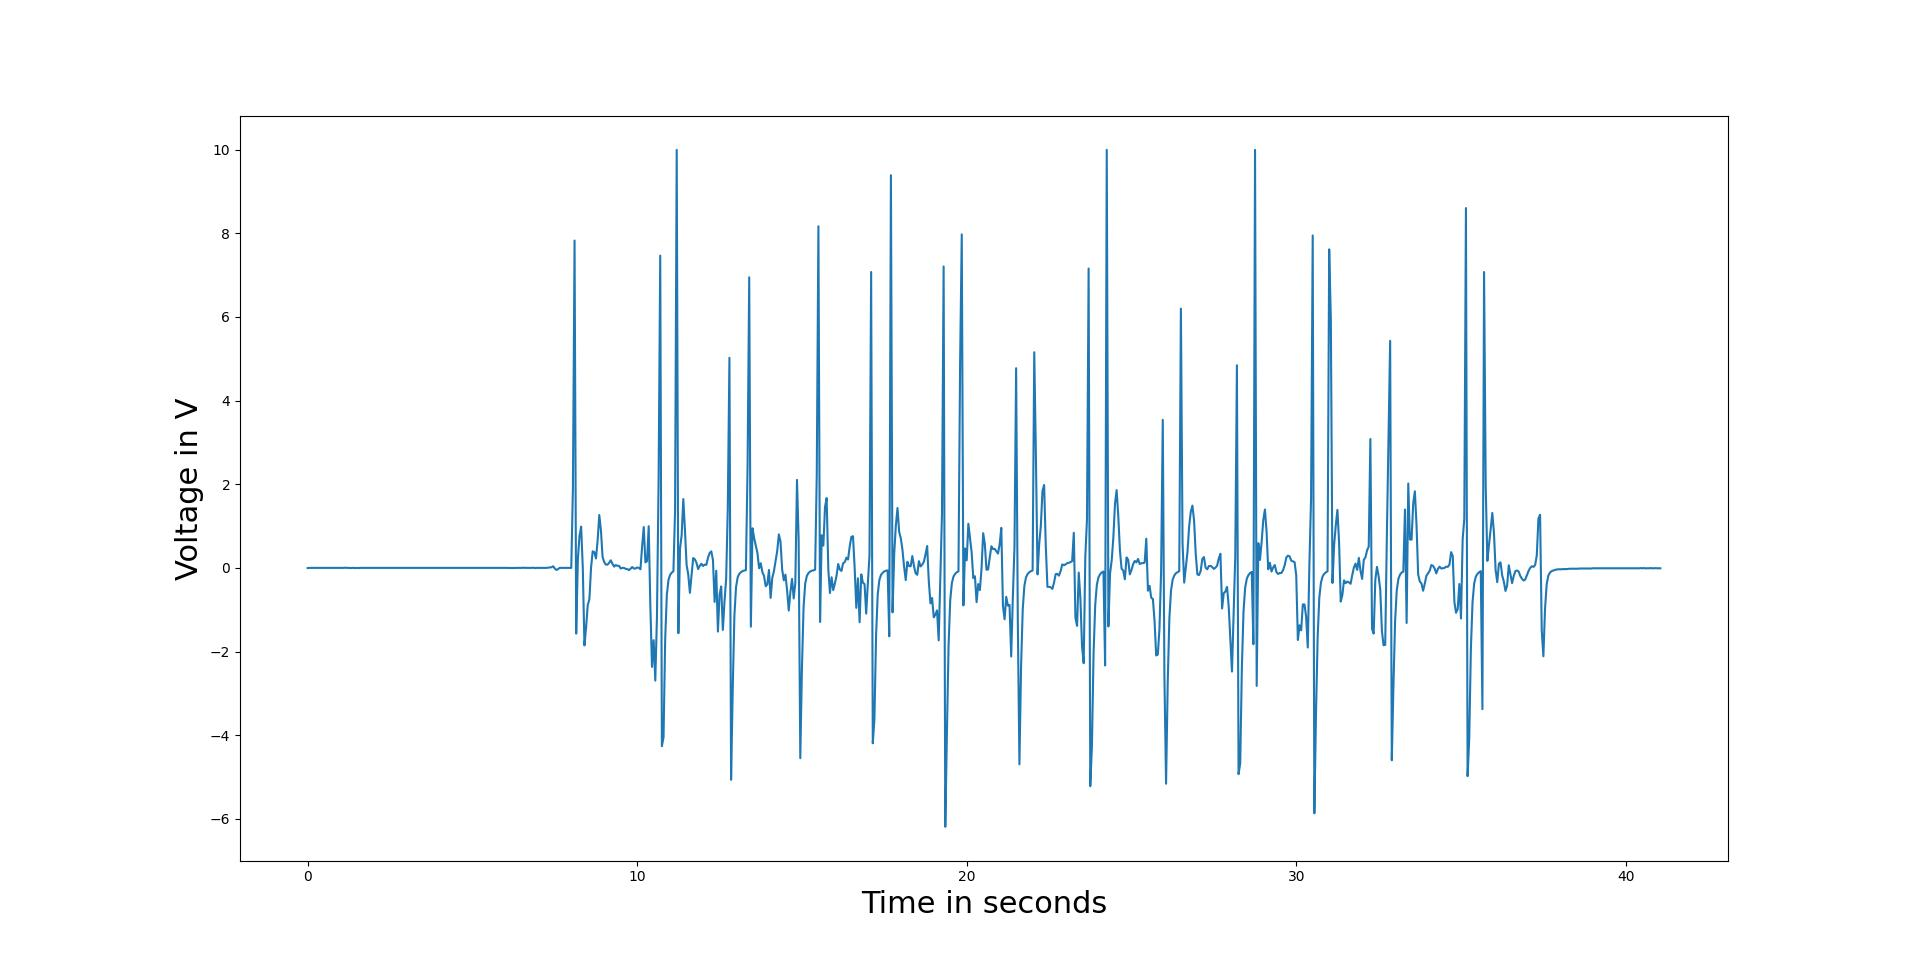
\includegraphics[width=\textwidth]{Figure_11.jpeg}
\captionof{figure}{Voltage Graph of Experiment}
\label{fig:Voltage Graph of Experiment}
\vspace{0.5cm}
When looking at the voltage graph (Figure \ref{fig:Voltage Graph of Experiment}) one can see that the voltage fluctuates between $-6.191 \pm 0.001$ and $9.995 \pm 0.001$ V. This is caused by the quartz expanding after being compressed. Since the quartz obeys the laws of conservation of energy the quartz crystal will not go back to its initial state but will overexpand. This causes the AC voltage. If DC voltage is needed a rectifier has to be used to convert AC into DC voltage.
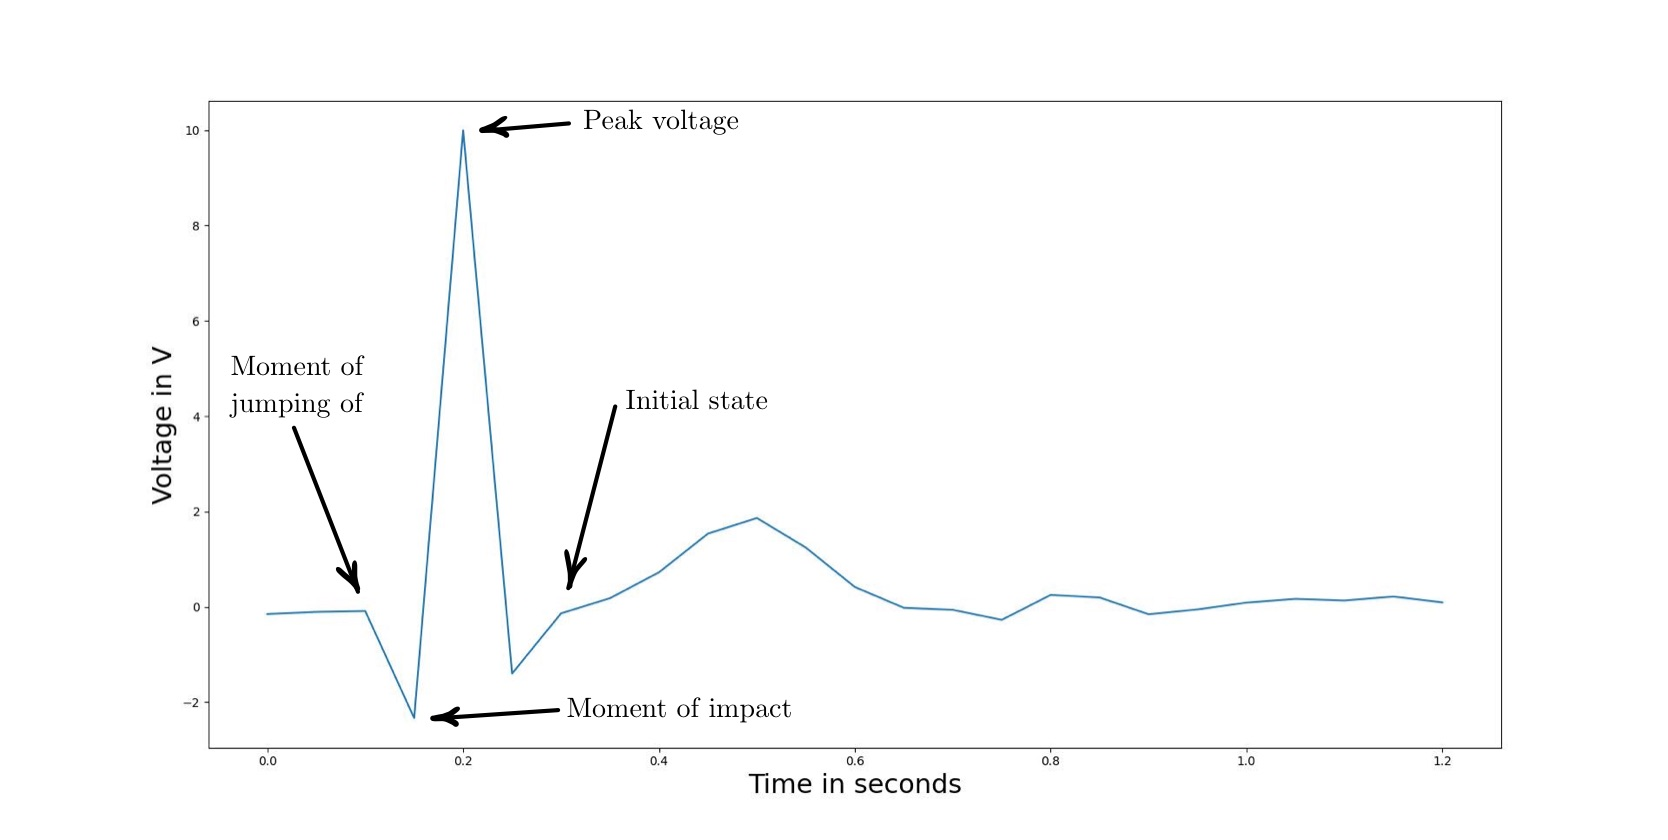
\includegraphics[width=\textwidth]{Figure_12.jpg}
\captionof{figure}{Section of the Voltage Graph}
\label{fig:Section of the Voltage Graph}
\vspace{0.5cm}
Having a look at Figure \ref{fig:Section of the Voltage Graph} one can see that the piezoelectric element undergoes many different stages. At first the piezoelectric element undergoes a expansion since the weight force is eliminated while jumping up. At the moment of impact, the piezoelectric element is compressed and a voltage can be meassured with its maximum being the peak voltage. Afterwards, the piezoelectric element decompresses going back to its initial state. %        \
\chapter{Theoretical Approach}

\section{Setup}

For the theoretical approach we consider a $1km$ long highway in Switzerland. The cars with a average weight of $1302 kg $ or $12772 N$ travel over this road. We estimate the wheel of the cars to have an average width of $22cm$ and an area of $0.0352m^2$ ground contact since the part of the wheel which touches the ground is about $4cm$ long.\cite{Kim2023}\\
In total, there will be $100000$ Piezoelectric elements connected in series planted into the road of size $22 \times 4 cm$ and a thickness of $0.133mm$ which was calculated by calculating the force needed to achieve $10 V$ with the piezoelectric element in the experiment. Afterwards the force was devided by the weight force of the car to get the constant by how much the the thickness had to be increased.
$$
F = \frac{10 \cdot 0.0088}{21.3 \cdot 10^{-3} \cdot 0.00022} = 21050 N
$$
$$
\frac{12772}{21050} = 0.6
$$
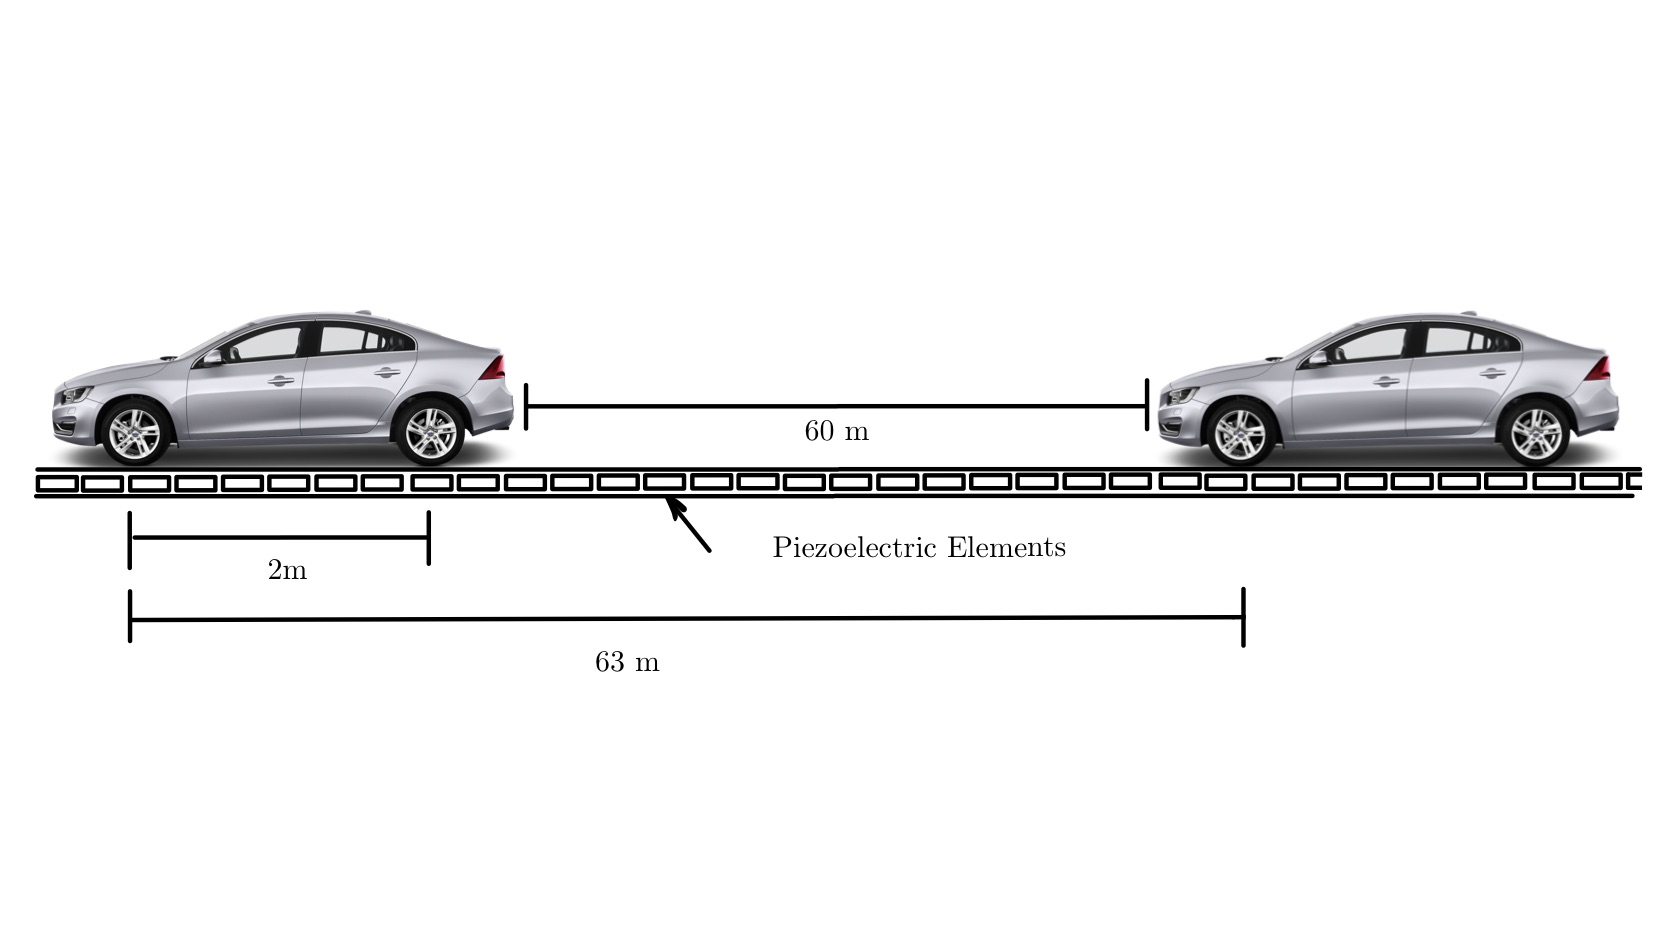
\includegraphics[width=\textwidth]{Figure_13.jpg}
\captionof{figure}{Setup of the Theoretical Approach}
\label{fig:Setup of Theoretical Approach}
\vspace{0.5cm}
A car is about $3m$ long in average and on the highway the cars have a distance of $60m$. Considering the fact that the wheels have a distance of $0.5m$ from the nose and tail of the car, the distance of the front wheel of the car infront will be $63m$ from the front wheel in the car in the back. (Figure \ref{fig:Setup of Theoretical Approach})\\

\section{Calculations}

So in an ideal scenario 15 cars can fit onto a $1km$ long road but not all of them have driven over the piezoelectric elements which also counts for the wheels. For the car in front only the front wheels have driven over all piezoelectric elements. The back wheels have driven over all except the last 100. This continues on for the next few cars.\\
This leads to the formula $2 \cdot \sum_{i=0}^{15} 4.51 \cdot (50000 - (i\cdot 1575)) + 4.51 \cdot (49900 - (i \cdot 1575))$ for the voltage since $V = 23.2 \cdot 10^{-3} \cdot \frac{12772 \cdot 0.000133}{0.0088} = 4.51V$, the amount of piezoelectric elements which the back wheels don't cover is 100, and the number of piezoelectric elements which the front wheels of the car in the back don't cover is 1575. In addition, there are two lanes hence we have to multiply the sum by 2. This leads to a output voltage of $11MV$.\\
For the energy, we can replace the voltage by the energy which is $E = \frac{1}{2} \cdot 1302 \cdot 9.81 \cdot \frac{1302 \cdot 9.81}{10^{10}} = 0.0081J = 2.27 \mu Wh$. This leads to $2 \cdot \sum_{i=0}^{15} 2.27 \cdot 10^{-6} \cdot (50000 - (i\cdot 1575)) + 2.27 \cdot 10^{-6} \cdot (49900 - (i \cdot 1575)) = 4.7Wh$
\chapter{Literature}

The concept of implementing piezoelectric elements in roads, railways, and highways has been around for a while now. That is why it is apparent that there has been much research done about this concept. However, there has been much skepticism about this concept regarding many aspects such as the costs and the energy harvested by the piezoelectric elements. On the one hand, a scientist from the company khplant predicts that 12 meters of road could produce 1 kWh when a car drives over it. There is also a team from Lancaster University, who are very confident about this concept and are preparing to deploy tests in the United Kingdom and Italy. They believe that they could harvest 1 – 2 MW per kilometer road. This seems very doubtful as on the other hand, Rex Garland from Stanford University claims that 1 km of read contains 1.54 MJ which is miles away from the 1 kWh or the 1 – 2 MW. Nonetheless, how much energy could a busy road produce?\cite{khplant2023,Garland2013}\\
In average, an electric car needs $10kWh$ for $80 - 100 km$ which is about $0.9kWh$ per $km$. This means that $12m$ of road produce a maximum of $0.012kWh$ which is far away from the $1 kWh$ promissed by the scientist from the company khplant. On the other hand, the thesis of the teams of the Lancester University is thesible if it is considered that 47-93 cars drive over this road per day and there is no loss in energy when it is converted.\\  
\\
There are also papers which praise the idea of piezoelectric elements in roads as a way to harvest energy. M. Vázquez-Rodriguez, F. J. Jiménez, and J. De Frutos published a paper in 2011 where they measured the voltage and power output a public road could create using a contraption and different piezoelectric materials. They concluded that the power output depended on the speed of the cars and the frequency with which the cars drive over the piezoelectric element. Nevertheless, the voltage only peaked between 0.455 and 0.900 Volts with $70 kg$ of force pressing onto the piezoelectric elements and the wheels having a velocity of $60 - 115km/h$. In the end, the paper also showed the estimated power output of $48.3 \mu W$ using the formula $P = \frac{V^2}{R}$. \cite{M.VAZQUEZRODRIGUEZ2011}\\
In the paper by Hiba Najini and Arumugam Muthukumaraswamy published in 2017, they used a DC-DC Booster in addition to the capacitor, which would increase the power output. Theoretically, they could have an output for a 1 km road of 187 kWh considering that there are 3280 piezoelectric elements implemented into the road and that there were 500 cars per hour travelling at 100 km/h. They also included theoretical calculations including the time where the traffic density was lower than 500 cars per hour. However, the energy outcome is imense ranging from 20.8 to 93.81 kWh. compared to the $0.9kWh$ a car produces with out loss of energy during the harvesting process. \cite{Najini2017} \\
According to Flurin Solèr's research paper from 2017, it had a similar result as the experiment of this paper. In fact, he was also limited by the maximum voltage output of the piezoelectric element. He measured the voltage output and calculated the theoretical power output a person could generate while walking. Even though the concept of generating power during walking sounds promising, he was only able to generate an estimate of 0.247 mW when walking $7km/h$. He also calculated that it would take 6.2 years to charge an iPhone with this method.\cite{Soler2017}\\ %     \
\chapter{Analysis and Conclusion}

\section{Analysis}

Looking at the theoretical calculations, the voltage seemed to be promising since the piezoelectric element is such a small device, which could produce a lot of voltage just by using pressure. Nevertheless, the theoretical calculation of the energy output showed, that the concept is nearly impossible to use in day-to-day life since the energy output would not be sufficient to power anything. Even if a car drove over the piezoelectric element, the energy harvested would not be sufficient. \\ 
The experiments also show similar results to the theoretical calculations. The calculated theoretical energy production of $7.4nWh$, leads to the fact that this energy cannot be used in daily life because tt is too little to be used as conventional electronical appliances use more energy.\\
Interestingly, the opinions about piezoelectric elements in roads, railways and pathways are quite split when looking at the papers. On the one hand, the papers show that the energy output is very little and not considerable to be used. On the contrary, the paper of Hiba Najini and Arumugam Muthukumaraswamy shows that the energy output can be significant, once a DC-DC  Booster is used and even profitable. Although considering the fact that 20 km of highway would be needed to energize a house in Switzerland for a whole year, the question arises whether it is worth implementing this concept in the highways of Switzerland. To put this into contrast, merely 4 houses could be energized if 500 cars travelled at a speed of 120 km/h from St. Gallen to Zurich.\\
So how can the piezoelectric element be used rather than as a source of energy? On the one hand, the piezoelectric elements could produce energy for a sensor measuring data. Furthermore, the piezoelectric element has better functionality when used as a sensor. One could monitor the voltage of the piezoelectric element to sense very little forces and even calculate the theoretical force. Moreover, the piezoelectric element can be used as a loud speaker since it vibrates according to specific voltages.\\ %      \
\section{Conclusion}

From the results of our research, one can derive two conclusions.\\
Firstly, one could observe that the piezoelectric element is limited by the maximum voltage output it can generate due to its thickness. This leads to the fact that the piezoelectric element will only produce its maximum voltage no matter how high the force is. Therefore, it is important to note that the formula is a theoretical approach to the voltage output of a piezoelectric element.\\
Finally, the experiment, the theoretical calculations, and the research papers showed that the power gained by the piezoelectric elements is not sufficient and not worth the costs as the revenue would not be profitable enough to cover the cost to implement piezoelectric elements. Furthermore, other sources producing renewable energy are far more profitable and generate more power. As for now, our technology is not sufficient for the use of piezoelectric elements as a source of renewable energy but perhaps in the near future, there will be a possibility where the piezoelectric element will function as a renewable energy source.\\
So, are piezoelectric elements a new renewable energy resource applicable in roads, railways, and pathways? Overall, the possibility of using piezoelectric elements as a renewable energy source is better understood. After simulating similar events where this concept could be used and understanding the limitations, one can now explain why this concept in our present will not be profitable enough to be used. Nevertheless, there are still many problems which have to be covered in this research.\\
The experiment is based on theoretical calculations due to the fact that the power produced is too small to be measured (Table \ref{Tab:Values of Power Graph 1}, \ref{Tab:Values of Power Graph 2}, \ref{Tab:Values of Power Graph 3}). In addition, the experiment is based on a very low frequency. This raises the question whether the theoretical calculations are applicable to the real results. Additionally, since the voltage output of the piezoelectric element used here is limited to 10 Volts, the experiment will never be able to provide the full potential of a piezoelectric element. This brings up the question whether the results from the experiment (Table \ref{Tab:Values of Voltage Graph 1}, \ref{Tab:Values of Voltage Graph 2}, \ref{Tab:Values of Voltage Graph 3}) are valid despite the theoretical calculated voltage having a discrepancy of $7.54 \pm 2.485 \%$ from the measured voltage. As we are limited to these materials, an experiment similar to the paper of M. Vázquez-Rodriguez, F. J. Jiménez, and J. De Frutos is not possible even though it would be more precise.\\
All in all, the research question could be answered. In our present time it is not worth implementing piezoelectric elements in roads, railways and pathways. Notwithstanding, its potential as a sensor is worth considering.
% --------------------------

% === Optional: INDEX ====
\cleardoublepage  %      \  
\phantomsection %        \
\addcontentsline{toc}{chapter}{\indexname} 
\printindex %            \
% ------------------------


% === ABBILDUNGSVERZEICHNIS ===
\cleardoublepage %             \
\phantomsection %              \
\addcontentsline{toc}{chapter}{\listfigurename}
\listoffigures %               \
% -----------------------------

% === CODEBLOCKVERZEICHNIS ===
\cleardoublepage %            \
\phantomsection %             \
\addcontentsline{toc}{chapter}{\lstlistlistingname}
\lstlistoflistings %          \
% ----------------------------

% === LITERATURVERZEICHNIS ===
\cleardoublepage %            \
\phantomsection %             \
\addcontentsline{toc}{chapter}{\bibname}
\printbibliography %          \
% ----------------------------



% =========== START VON ANHÄNGE ===========
\appendix

% ----------------------------------

% =========== ENDE VON ANHÄNGE ============



% =============================================================
\end{document} % ENDE VOM DOKUMENT ============================
% =============================================================















\documentclass[a4paper,11pt]{report}

\usepackage{amsmath}
\usepackage[naturalnames]{hyperref} % Hyperlinks im PDF-Dokument.
% Auf Windows-Systemen vor Windows 7 
% ist latin1 anstatt utf8 zu verwenden.
% Danach vielleicht auch noch...
\usepackage[utf8]{inputenc} % Codierung dieser Datei

\usepackage[german]{babel} % Falls nötig, Sprache anpassen.
\RequirePackage{lmodern} % Schrift, damit Schweizer Anführungszeichen
                         % << >> funktionieren.
\usepackage{fancyhdr}    % Header und footer
\usepackage{setspace}    % 1.5 Zeilenabstand
\usepackage{graphicx}    % Grafiken (png oder pdf)
\usepackage{verbatim}    % Text ohne Formatierung ausgeben
\usepackage{color}       % Farbiger Text (nicht wirklich empfohlen)

\usepackage{makeidx}     % Optional, für Glossar (Index)
\makeindex

\usepackage{geometry}    % Ränder festlegen
\geometry{
  a4paper,
  total={150mm,237mm},
  left=25cm,
  top=25mm,
}
\usepackage[normalem]{ulem} % Strikethrough text

% Hack für Titel
\author{{\sc Ivo Blöchliger}\\[4cm]
\includegraphics[width=5cm]{ksbglogo.pdf}\\[1cm]}
\title{\LaTeX{}-Vorlage für Maturarbeiten}
\date{34. Oktember 2016\\[3cm]Betreuer\\ {\sc Dr. Ivo Blöchliger}}



\newcommand{\atan}{\ensuremath{\mathrm{atan2}}}

\begin{document}

\maketitle %Diese Seite soll vielleicht besser selbst gestaltet werden
%\pagestyle{empty}
%Keine Seitennumer für das Inhaltsverzeichnis
%\fancypagestyle{empty}
%\fancyhf{} % clear all header and footer fields

%\setcounter{page}{2} % Inhaltsverzeichnis ist auf Seite 2


% Inhaltsverzeichnis anlegen (mit normalem Zeilenabstand)
\tableofcontents

\newpage % Neue Seite
% Zeilenabstand 1.5
\onehalfspacing

% Header definieren, je nach Geschmack.
\renewcommand{\chaptermark}[1]{\markboth{\MakeUppercase{\thechapter.\ #1}}{}}
\renewcommand{\sectionmark}[1]{\markright{\thesection.\ #1}{}}
\fancyhead[R]{\rightmark}
\fancyhead[L]{\leftmark}
\fancyhead[C]{- \thepage{} -}
\fancyhead[L]{\leftmark}
\fancyhead[R]{\rightmark}
\fancyfoot{}

\pagestyle{fancy}

%Keine Nummer für das Vorwort, darum manuell
%ins Inhaltsverzeichnis eintragen.
\chapter*{Vorwort}\addcontentsline{toc}{chapter}{Vorwort}
\section*{TODO}
Umstellen von {\tt bibtex} auf {\tt biblatex}. Anfügen einer Danksagung.

{\tt usepackage autoref}: Automatische Referenzen (mit Kapitel, Seite). Bei biblatex dabei.

Bildpfad generell festlegen.

PDF-Metadaten.

Das ist $\atan$. Zeigen, wie man neue Kommandos definiert.

Ablauf Kapitel besser definieren.
%Einbinden weiterer tex-Dateien (um etwas Ordnung zu haben)
\input{einleitung}
\input{literatur}
\input{grafiken}
\input{compilieren}
\input{mathezeugs}
\input{code}

%\input{danksagung}

% Optional, Index
\cleardoublepage
\phantomsection
\addcontentsline{toc}{chapter}{\indexname}
\printindex

% Abbildungsvereichnis
\cleardoublepage
\phantomsection
\addcontentsline{toc}{chapter}{\listfigurename}
\listoffigures


% Literaturverzeichnis
%
% Stil der Literaturangaben festlegen
% siehe
% http://amath.colorado.edu/documentation/LaTeX/reference/faq/bibstyles.html
% für eine Übersicht
\bibliographystyle{amsplain}
% Name des zu verwendenden .bib-files (oder mehrere, durch Kommata getrennt).
\cleardoublepage
\phantomsection
\addcontentsline{toc}{chapter}{\bibname}
\bibliography{literatur}

\appendix
\chapter{Eigenständigkeitserklärung}
<<I confirm with my signature that I have written my Extended Essay independently and put it into written form, that the involvement of other persons has been limited to consultation and proofreading, and that all documents and guarantors used are listed. I am aware that a Exteded Essay which is proven to be plagiarism according to the definition given in the Extended Essay Brochure will be considered a serious violation in the sense of the International Baccalaureate Examination Regulations.>>
\vspace{3cm}

\noindent
\begin{tabular}{p{0.47\linewidth}p{0.47\linewidth}}
  Place \&\ Date & Signature \\
  & \\[1cm]
  \hline
\end{tabular}


\end{document}
